
\documentclass[review,3p,times,authoryear,12pt]{elsarticle}

\usepackage{subfigure}
\usepackage{amsmath, amsthm, amssymb}

\usepackage{graphicx}
\usepackage{algorithm}
\usepackage{algorithmic}
\usepackage{clrscode3e}
\usepackage{url}
\usepackage{multirow}
\usepackage{longtable}
\usepackage{color}


\journal{TBD}
\newtheorem{corollary}{Corollary}
\newtheorem{theorem}{Theorem}
\newtheorem{definition}{Definition}
\newtheorem{proposition}{Proposition}
\newtheorem{lemma}{Lemma}
\begin{document}
\graphicspath{{./figure/}}
\begin{frontmatter}
\newpage

\title{Target guided algorithms for the container pre-marshalling problem}

\author{Ning Wang}
\ead{wangning@cityu.edu.hk}

\author{Bo Jin\corref{corl}}
\ead{msjinbo@cityu.edu.hk}

\author{Andrew Lim}
\ead{lim.andrew@cityu.edu.hk}

\address{
Department of Management Sciences, City University of Hong Kong, 83 Tat Chee Ave, Kowloon Tong, Hong Kong
}
\cortext[corl]{Corresponding author. Tel: +852 34425296}

\begin{abstract}
We investigate the container pre-marshalling problem (CPMP), which aims to rearrange containers in a bay with the least movement effort, so as to find a final layout where containers are piled according to a predetermined order. Previous researchers, without exception, assume that all the stacks in a bay are functionally identical. We reexamine such a classic problem setting and propose a new problem -- the CPMP with a dummy stack (CPMPDS).
At terminals that use gantry cranes, a bay includes a row of ordinary stacks and a dummy stack. The dummy stack actually is the bay space reserved for trucks, via which containers can be shipped out of the bay. During the pre-marshalling process, the dummy stack temporarily stores containers, just like an ordinary stack.
But it is required to restore emptiness at the end of the pre-marshalling process. In this paper, we propose target guided algorithms to tackle both the classic CPMP and the new CPMPDS; the key idea is to fix containers at appropriately chosen positions one by one. We also devise an improved lower bound for the number of required movements. Experimental results in terms of the CPMP showcase that our algorithms surpass the state-of-the-art algorithm.
\end{abstract}

\begin{keyword}
container pre-marshalling \sep target guided algorithms\sep lower bound \sep dummy stack
\end{keyword}
\end{frontmatter}

\section{Introduction}

Seaborne transportation is the cornerstone of international trade and undoubtedly an engine of global economic development. According to \textit{Review of Maritime Transport} (2012) released by UNCTAD, around 80\% of global trade by volume is carried by sea. Amongst different ship types, container ships account for about 62\% of dry cargoes. Since the commencement of containerization, containers facilitate smooth flow of goods across multiple transportation modes without direct handling the freight during the course of shipping. Accompany with the rapid growth of container shipping, container terminals face unprecedented development opportunities.
The role of container terminals lies in providing physical spaces for container exchanges between sea and land. At terminals, a large proportion of land spaces is reserved for storing containers temporarily, which is known as container yards. A yard acts as a cache that makes the loading and unloading process of ships in a fast pace. Basically, a conventional practice of exporting containers is to store them on the yard first. When the ship arrives, all the containers are transported by trucks to the quayside and then loaded onto the ship. The process is reverse for import containers.

High efficiency is a key factor for any successful terminals since shipping line managers prefer efficient terminals. Carriers or shippers bear the pressure of quick delivery from down stream customers. Moreover, high efficiency increases the turnover rate of terminals, therefore generates more profit for the shareholders. Container terminals have every reason to increase their operational efficiency as much as possible. Both terminal practitioners and OR researchers have paid considerable attention on improving the efficiency of quayside operations. Nonetheless, the overall terminal productivity will not increase dramatically if only quayside operations are optimized, leaving yard operations inefficient \citep{Jiang2012}.

In general, a yard is divided into several blocks and a block is composed of several parallel bays. Each bay is formed by several stacks aligned side by side. In each stack, containers are piled vertically. Figure \ref{fig:1} shows a diagram of a yard. The height of stacks is constrained by the height of operation equipments, i.e. gantry cranes. Generally speaking, one stack can store 3$\sim$10 containers.

\begin{figure}[htbp]
\centering
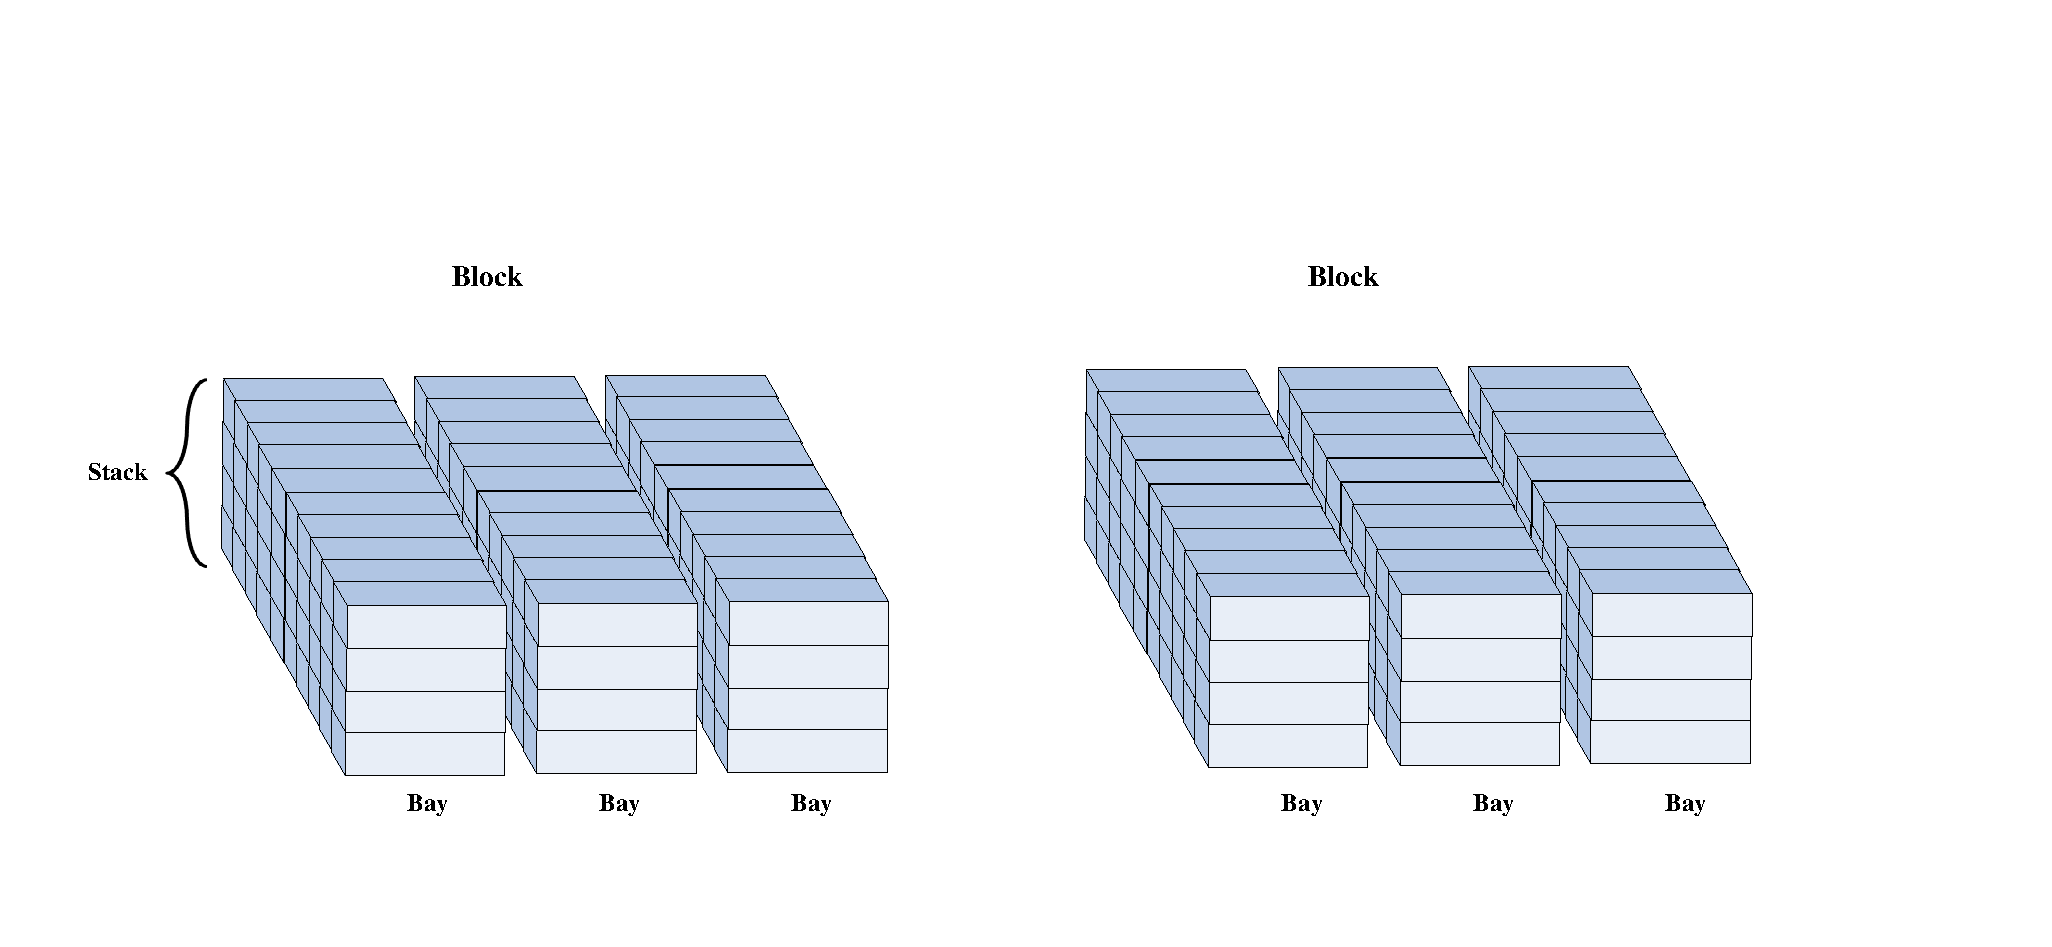
\includegraphics[width=0.60\textwidth]{fig1.pdf}
\caption{An example of a container yard}
\label{fig:1}
\end{figure}

Containers in the same stack can only be retrieved in a ``first in last out'' manner. If the container to be fetched is not at the top of a stack, all the containers placed above it have to be relocated to other stacks before retrieving it. Such forced movements are known as rehandlings. Rehandling containers is a costly activity as this additional work decreases the efficiency of container retrieval, whereas consignors do not pay for this. In the ideal situation, containers are piled in an order consistent with the retrieval order, i.e., containers retrieved earlier are located at higher tiers. The realistic situation, however, goes by contraries. The placement order of containers is decided by inland transportation or consignors; while the retrieval order of containers is decided by the stowage planning or ship schedule. In most situations, the two orders are not exactly reverse. In reality, containers which arrive early do not necessarily depart late.

Prior to ship arrival, containers in a bay can be rearranged to comply with their retrieval order, hence the name pre-marshalling. The pre-marshalling work, though not billable to consignors, can reduce the berthing time of ships and increase the turnover rate of terminals. How to carry out the container pre-marshalling with the least effort is the so called container pre-marshalling problem (CPMP).
%In the CPMP, a set of containers piled in a bay are given, and each container is assigned with a group label which represents its retrieval batch ordinal. A movement can only move a container from the top of a stack to the top of another stack, resulting in a new layout. The objective of the CPMP is to find the shortest movement sequence which rearranges containers and pile them according to the descending order of group labels from the bottom up.

%One conventional objective is to minimize the number of movements. Gantry movement is a reasonable indicator, as gantry cranes can only process $20 \scriptsize{\sim} 25$ container movements per hour \cite{Rotter2004}, which suggests that gantry cranes are definitely a kind of valuable resource.


By far, though the research community has studied the CPMP, it does not fully depict practical scenarios. For terminals using gantry cranes, the bay must reserve extra space for trucks beside stacks in the bay, so that trucks can stand by and receive containers from the handling equipments, just as shown in Figure \ref{fig:2}.\footnote{Photo by \url{http://www.saifpowertecltd.com/port_operation.php}} When no container is being retrieved, the extra space acts as a temporary stack for the pre-marshalling work just like an ordinary stack. The only issue demanding attention is that the extra space should become empty again after the pre-marshalling work, which distinguishes itself from ordinary stacks. We coin the extra space as a \textbf{dummy stack}.
%If regarding the extra space as a dummy stack, the initial layout is composed of several (nearly) fully occupied stacks, together with an empty dummy stack.

\begin{figure*}[htbp]
\centering
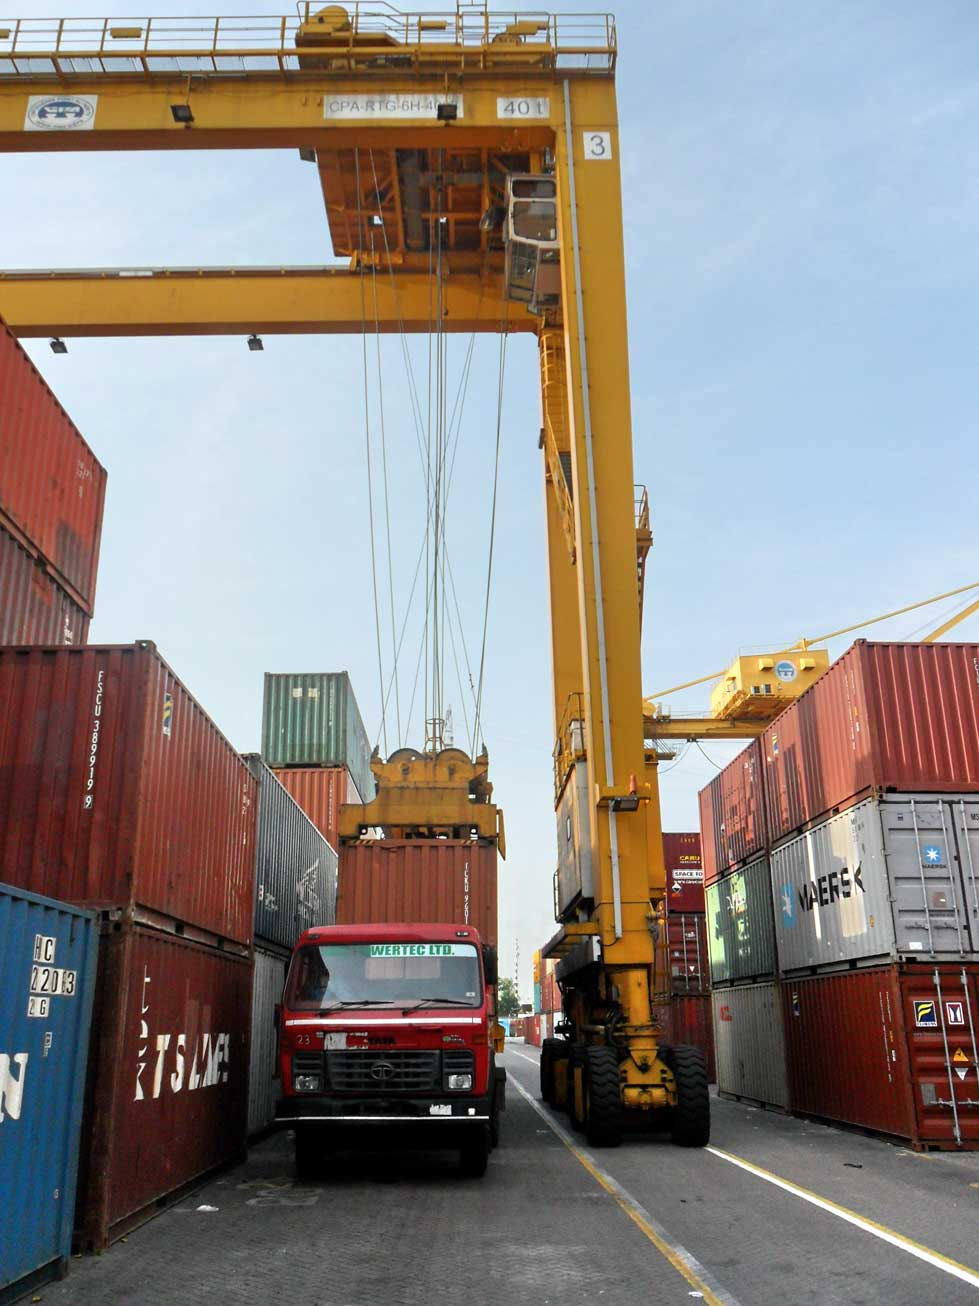
\includegraphics[width=0.3\textwidth]{fig2.jpg}
\caption{A container bay and a truck}
\label{fig:2}
\end{figure*}

Existing algorithms for the CPMP have not taken the dummy stack into consideration, hence they cannot be implemented directly at terminals using gantry cranes. However, terminals using gantry cranes as yard operation equipments are rather popular across the world. Herein, it is imperative to fill this disparity between research and industry.

Our paper contributes to the literature on three aspects. We reexamine the CPMP and propose a new variant -- the CPMP with a dummy stack (CPMPDS). We devise a new lower bound on the calculation of movements, suitable for both CPMP and CPMPDS. The new lower bound dominates other existing lower bounds with respect to the CPMP. In addition, we design three algorithms innovated by the idea of target-guided to solve both the classic CPMP and the new CPMPDS which cannot be solved by existing algorithms directly. The ideology of the algorithms is to fix containers at appropriately chosen positions and avoid moving them afterwards. This mechanism reduces the problem size continuously until the problem is solved. Experimental results demonstrate that our algorithms are better than the state-of-the-art algorithm to the best of our knowledge. It is noteworthy that although this paper discusses the CPMP in the context of maritime terminals, it is also applicable to other scenarios such as warehouses and railway yards.

The remainder of this paper is structured as follows. Section \ref{sec:litreview} presents an overview of existing works related to the CPMP. After that, we formally define the CPMP/CPMPDS in Section \ref{sec:pd} and present how to check instances feasibility in Section \ref{sec:cf}. A heuristic algorithm and two advanced beam search algorithms are elaborated in Section \ref{sec:heu} and Section \ref{sec:g2la} respectively. We conduct experiments which evaluate the effectiveness of our algorithms and report the results in Section \ref{sec:ce}. At last, we conclude our research in Section \ref{sec:con} with some closing remarks.

\section{Literature review}
\label{sec:litreview}

In recent years, publications in press concerning maritime transportation, especially container transportation, have exploded. \cite{Vis2003} are the first who give an overview of the complex operations at container terminals and associated research problems.
Then \cite{Steenken2004} provide a more extensive description on main logistics processes and operations at container terminals, together with a corresponding survey of optimization models and methods. It is followed by \cite{Stahlbock2008} who trace new updates on container terminals.
Collectively, these studies point out that the CPMP is an important topic and worthy of more research effort.

Most existing methods for the CPMP are heuristic approaches. \cite{Caserta2009} provide a greedy heuristic based on the paradigm of corridor and roulette wheel. The corridor reduces the number of movement choices for a certain layout and the roulette wheel brings randomness when making choices. The probability of selecting an alternative is proportional to the corresponding attractiveness.
Their algorithm first builds a corridor with respect to the current layout to determine the destination stacks of a specific misplaced container. Then it yields new layouts by conducting the movements in the corridor, and evaluates the attractiveness of each new layout by an estimated number of needed relocations. It also conducts a local improvement scheme to accelerate the search process.
\cite{Exposito2012} propose a multi-start heuristic to minimize the number of rehandlings. They select movements by a rule called ``low priority first'', so their method is more target-oriented than the one of \cite{Caserta2009}. In their work, the concept of corridor and roulette wheel are also used when building solutions. What is more, they give a method to generate instances and measure the difficulty of an instance.

Different from the above approaches that construct solutions by finding promising movements step by step, \cite{Lee2009} deploy a neighborhood search where complete solutions are regarded as the units of search. The neighborhood search obtains a new feasible solution by randomly modifying the current solution.
Solutions are further shortened without disturbing the feasibility by a four-step procedure. In addition, three minor routines are devised to diversify the resultant solutions and further reduce the number of movements. As it is very likely to generate infeasible solutions by pure modification, their method needs a large number of iterations. Hence, it is not as efficient as the heuristic of \cite{Exposito2012}.
After that, \cite{Huang2012heu} solve two variants of the CPMP by a heuristic algorithm. One variant is commonly seen which allows containers of different groups to mix within a bay; while the other variant is newly proposed which requires containers of different groups separately located in the final layout.

Apart from heuristics, \cite{Lee2007} develop an integer programming model to tackle the CPMP. They convert the CPMP into a multi-commodity network flow problem. A network is composed of several subnetworks, with each representing an interim layout.
The nodes in a subnetwork correspond to the slots of the bay while the containers are expressed as the commodities. A solution is expressed by a flow in the network. The disadvantage of their algorithm is that the scale of networks is giant even for small instances.
Whereas, it provides us an innovative view to investigate the CPMP.
\cite{BF2012} thoroughly describe a tree search procedure and a new lower bound for the CPMP. In the search tree, solutions are constructed by compound moves (several movements) instead of single movements, and the branches are classified by four movement types. Their performance, by far, is the best among all the extant methods.
%\cite{Vob2012} gives a short note discussing an improved lower bound on the number of required container movements.

As discussed in \cite{Caserta2011}, the counterparts of the pre-marshalling problem include the container re-marshalling problem and the container relocation problem. The container re-marshalling problem refers to reassigning containers scattered within a block into their designated bays. It is not a simple extension of the CPMP, as there are multiple cranes involved. The interference between multiple cranes, as well as the stacking positions of containers within a bay, is the difficulty of the problem.
\cite{Caserta2011}, in their paper, prove that the container re-marshalling problem is NP-hard. \cite{Kim1998, Kang2006Plan, Park2009Plan, Choe2011} have exploited the container re-marshalling problem and came up with some heuristic methods to cope with it. On the other hand, the container relocation problem aims to retrieve containers in a predetermined order with the fewest movements. It has been studied by researchers using various methods, ranging from meta-heuristics to simple heuristic algorithms \citep{Kim2006A, Yang2006A, Caserta2009A,Caserta2009Applying,Lee2010A,Caserta2012AM, Forster2012A, Zhu2012Iter}.


%Pre-marshalling is the preliminary work for the
%ship stowage (rf. Avriel et al. (1998) and Imai et al. (2006)); container priorities are decided by the containers
%loading order in the ship stowage.
%
%\cite{Meisel2010Con} investigate the container sequencing problem in a vessel bay. In their problem, inbound and outbound containers are exchanged between the vessel bay and yard, and they try to determine the container handling sequence so as to minimize the container handling time.
%
%\cite{Castilho1993Handling, TalebIbrahimi199313} analyze the effect of storage space and stacking strategies on the expected number of rehandles. \cite{Kim1999Segregation} deal with how to decide the height of stacks for import containers in a dynamic setting. Their objective is to minimize the number of rehandles. \cite{Kim2000} suggest a methodology to determine storage slots for every exported container in a bay while considering container weights and the layout of the bay with the objective to minimize the anticipated number of rehandles. \cite{Kang2006} propose a simulated annealing search to reduce the number of relocation movements of export containers with inaccurate weight information at the time of loading. In this work, a reduction on the number of relocations is obtained by applying a learning classifier.

\section{Problem description}
\label{sec:pd}

The container pre-marshalling problem (CPMP) can be summarized as follows: given a bay with $S$ stacks, each stack is able to store up to $H$ containers vertically. Tiers of the bay are indexed from 1 to $H$ from the bottom up. To make it consistent, the ground is considered as tier 0 in particular.
There are $N$ ($N\le S\times H$) containers stored in the bay, forming the initial layout with a usage rate $N/(S\times H)$. Each container $c$ is assigned with a group label $g(c)\in \{1,\dots,G\}$, and the group label of different containers could be unique or duplicate. Figure \ref{fig3} shows an example of a layout.

One container can be moved from the top of a stack (\textbf{origin}) to the top of another stack (\textbf{destination}) if the destination stack is not fully occupied.
The CPMP is to find the shortest movement sequence which transforms the initial layout to a final layout with all the stacks \textbf{clean}. A stack is \textbf{clean} if its containers are piled in a non-increasing order of group labels from the bottom up, otherwise we say it is \textbf{dirty}. We say a stack $s$ can \textbf{accommodate} a container $c$ if and only if stack $s$ is clean and is still clean if moving container $c$ to its top.
A container $c$ in a certain layout is a clean container if and only if all the containers underneath are clean and their group labels are no smaller than $g(c)$. Otherwise, it is a dirty container.


\begin{figure*}[htbp]
\centering
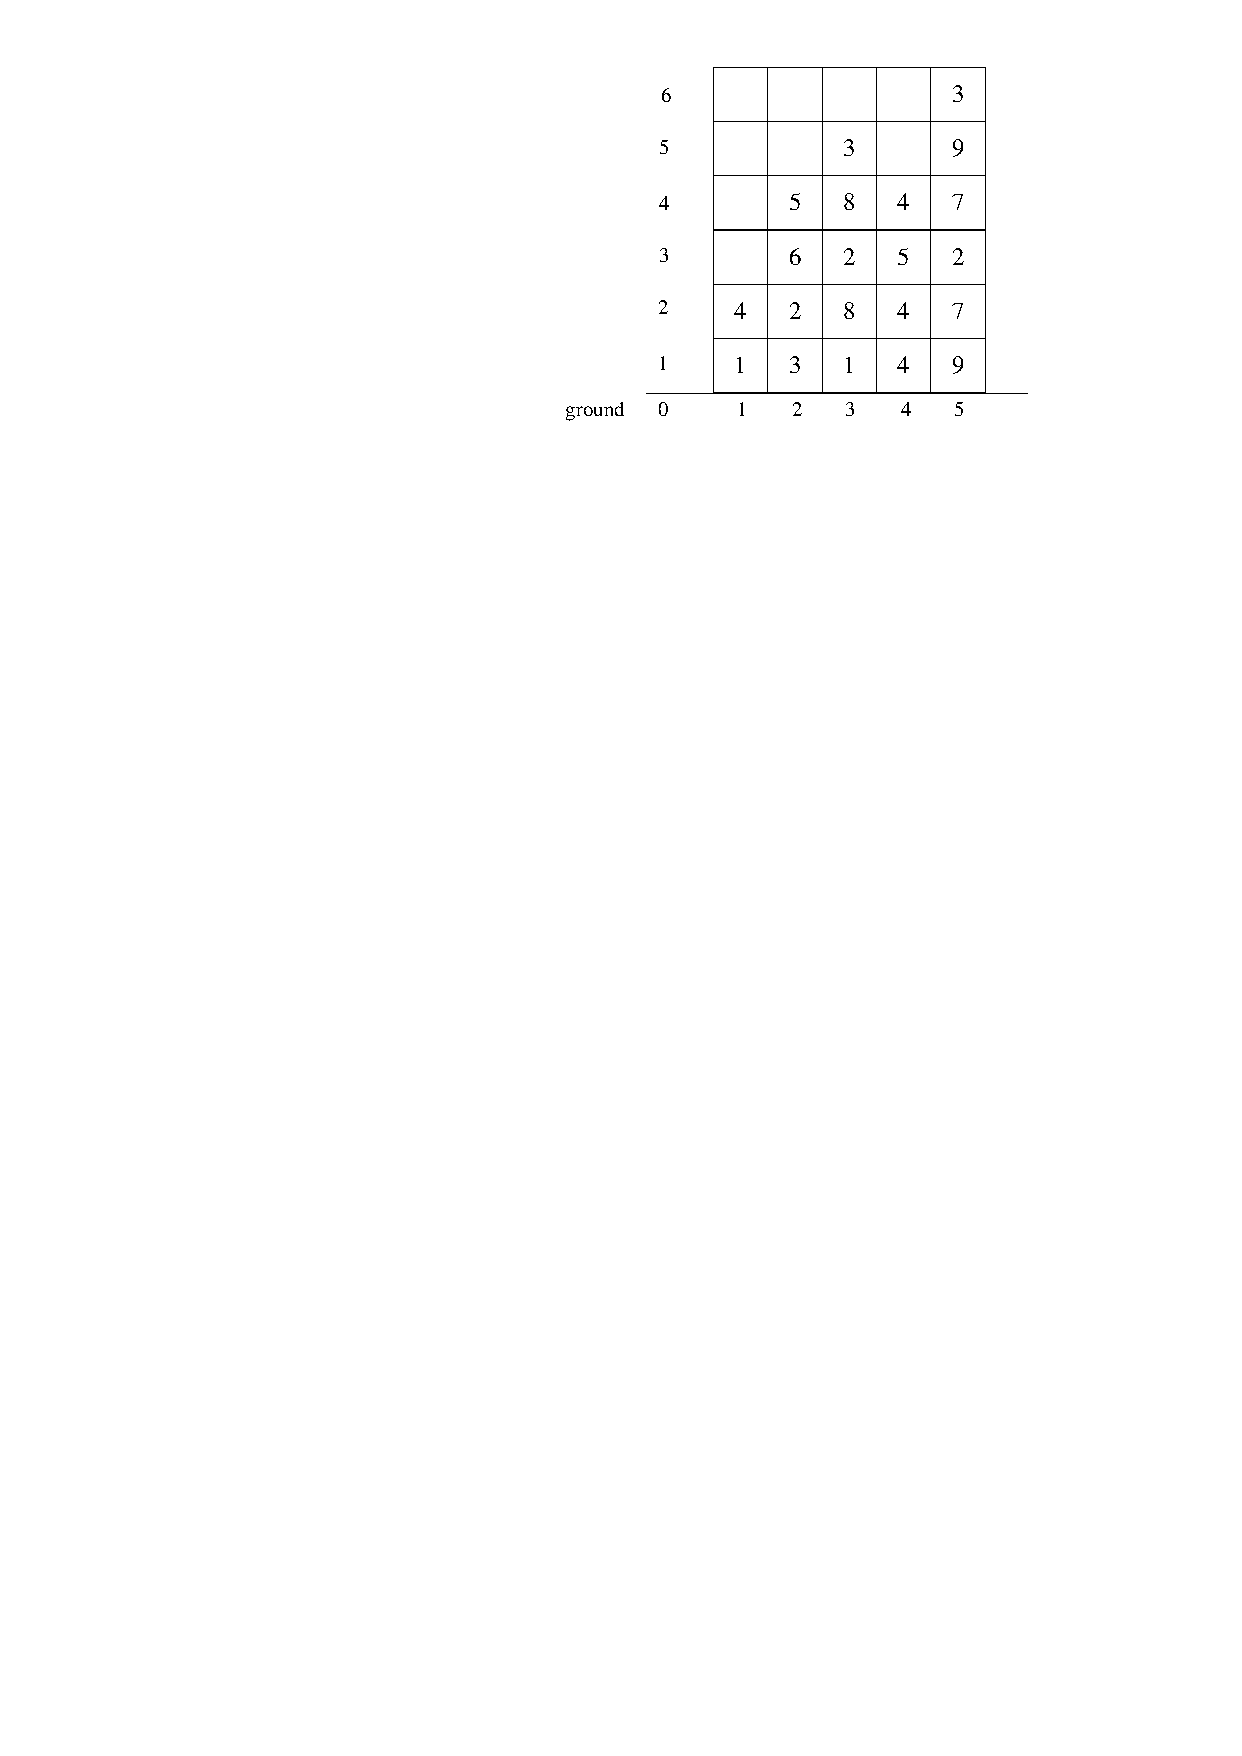
\includegraphics[width=0.4\textwidth]{fig3.pdf}
\caption{An example of a layout}
\label{fig3}
\end{figure*}

%Our paper uses the following assumptions which have been presented in \cite{Lee2007} for the resolution of the CPMP:
%\begin{enumerate}[1.]
%\item Container movements are only carried out within a single bay, i.e. movements across bays are not considered here.
%\item All the containers have the same dimensions. This is the conventional practice in container terminals.
%\item Container group labels are known in advance and do not change over time, as the ship stowage plan is determined prior to the pre-marshalling process.
%\item No container comes in or goes out of the bay when the pre-marshalling process is performed in the bay.
%\end{enumerate}

In the new variant -- the container pre-marshalling problem with a dummy stack (CPMPDS), containers are only piled in the first $S-1$ stacks, while the $S$-th stack (so called dummy stack) is empty in the initial layout. During the course of pre-marshalling, containers can be placed in the dummy stack. The objective of the CPMPDS is to transform the initial layout to a clean layout where the dummy stack is empty, with the least movement effort.

For ease of illustration, we define some notations in Table \ref{tab:1}. All of the notations are used in the context of the current layout, therefore we do not explicitly point out the layout in notations.

\begin{table}[htbp]
  \centering
  \caption{Notations}
  \label{tab:1}
    \begin{tabular}{l|l}
    \hline
    Notations         & Description \\
    \hline
    $H$               & The height limitation of the bay\\
%    $s_i$             & The $i$-th stack\\
%    $c_j$             & The $j$-th container\\
%    $l_k$             & The $k$-th layout; the initial layout is $l_0$\\
    $e(s)$            & The number of empty slots of stack $s$\\
    $h(s)$            & The number of containers piled at stack $s$\\
    $d(s)$            & The number of dirty containers of stack $s$\\
    $\id{uf}(s)$      & The number of unfixed containers of stack $s$\\
    $\id{sn}(c)$      & The stack in which container $c$ is placed\\
    $\id{tn}(c)$      & The tier at which container $c$ is placed\\
    $g(c)$            & The group label of container $c$\\
%    $\langle c,s\rangle$           & A movement which moves container $c$ to the top of $s$\\
  % $(c_1,s_1)\circ\dots\circ(c_k,s_k)$ & A movement sequence with $k$ movements\\
    $o(c)$          & The number of containers above $c$\\
    \hline
    \end{tabular}
\end{table}



%A movement $\langle c, s\rangle$ can be applied (carried out) to a layout $l$ if and only if $s\neq \id{sn}(c,l)$, $h(s,l)<H$ and $c$ is the topmost container of a stack in $l$.
%The resultant layout is represented by $l\circ\langle c,s\rangle$. Analogically, $l \circ\langle c_1,s_1\rangle \circ \dots \circ \langle c_k,s_k\rangle$ represents the resultant layout after applying a sequence of movements $\langle c_1,s_1\rangle$, \dots, $\langle c_k,s_k\rangle$ to $l$.

%In addition, we classify the container movements into four types, just like \cite{BF2012}. A movement is a dirty-clean (DC for short) movement if a container is moved from a dirty stack to a clean stack. Similarly, the other three types are dirty-dirty  (DD), clean-dirty (CD), and clean-clean (CC). Generally, dirty-x (DX) denotes either DC or DD movements.

\section{Feasibility check \& lower bound}
\label{sec:cf}

In this section, we discuss how to check the feasibility of a CPMP/CPMPDS instance. We just briefly depict the check method here, since it is originally raised by \cite{Wang2013Check}. For a more comprehensive explanation and proof, please refer to the aforementioned paper.

\subsection{Movable and immovable containers}
We first recall the definition and conclusions in \cite{Wang2013Check} to make the content self-contained.

\begin{definition}
\label{def:1}
A container is movable if it can be fetched and replaced to another stack.
\end{definition}

In a given layout, for any stack $s$, only the top $\sum\limits_{i\neq s}e(i)$ containers are movable. Other containers in stack $s$, if any, are immovable.

\begin{lemma}
\label{lem:1}
Given a layout, the numbers of immovable containers in every stack are the same, equal to
\begin{equation}
\id{im}=\max\left\{0, H-\sum_{s=1}^S e(s)\right\}
\end{equation}
\end{lemma}
\begin{proof}
The proof of Lemma \ref{lem:1} can be found in \cite{Wang2013Check}.
\end{proof}

\begin{theorem}
\label{the:1}
Given a layout with $S\ge3$, movable containers can be rearranged in any order within the whole bay.
\end{theorem}
\begin{proof}
The proof of Theorem \ref{the:1} can be found in \cite{Wang2013Check}.
\end{proof}

Based on Theorem \ref{the:1}, we know that movable containers can be moved freely while immovable containers cannot be moved at all. According to Lemma \ref{lem:1}, we can separate movable containers and immovable containers at the beginning and the separation will never change, no matter what movement sequences are executed in later stages.
Since the numbers of immovable containers in every stack are the same, if we draw a boundary line between movable and immovable containers, the line is just horizontally straight (Figure \ref{fig4}).
%We define the slots above the boundary line as \textbf{movable slots} and the slots beneath the boundary line as \textbf{immovable slots}.

\begin{figure}[htbp]
\centering
\subfigure[Case 1]{
    \label{fig4:1}
    \resizebox{0.3 \textwidth}{!}{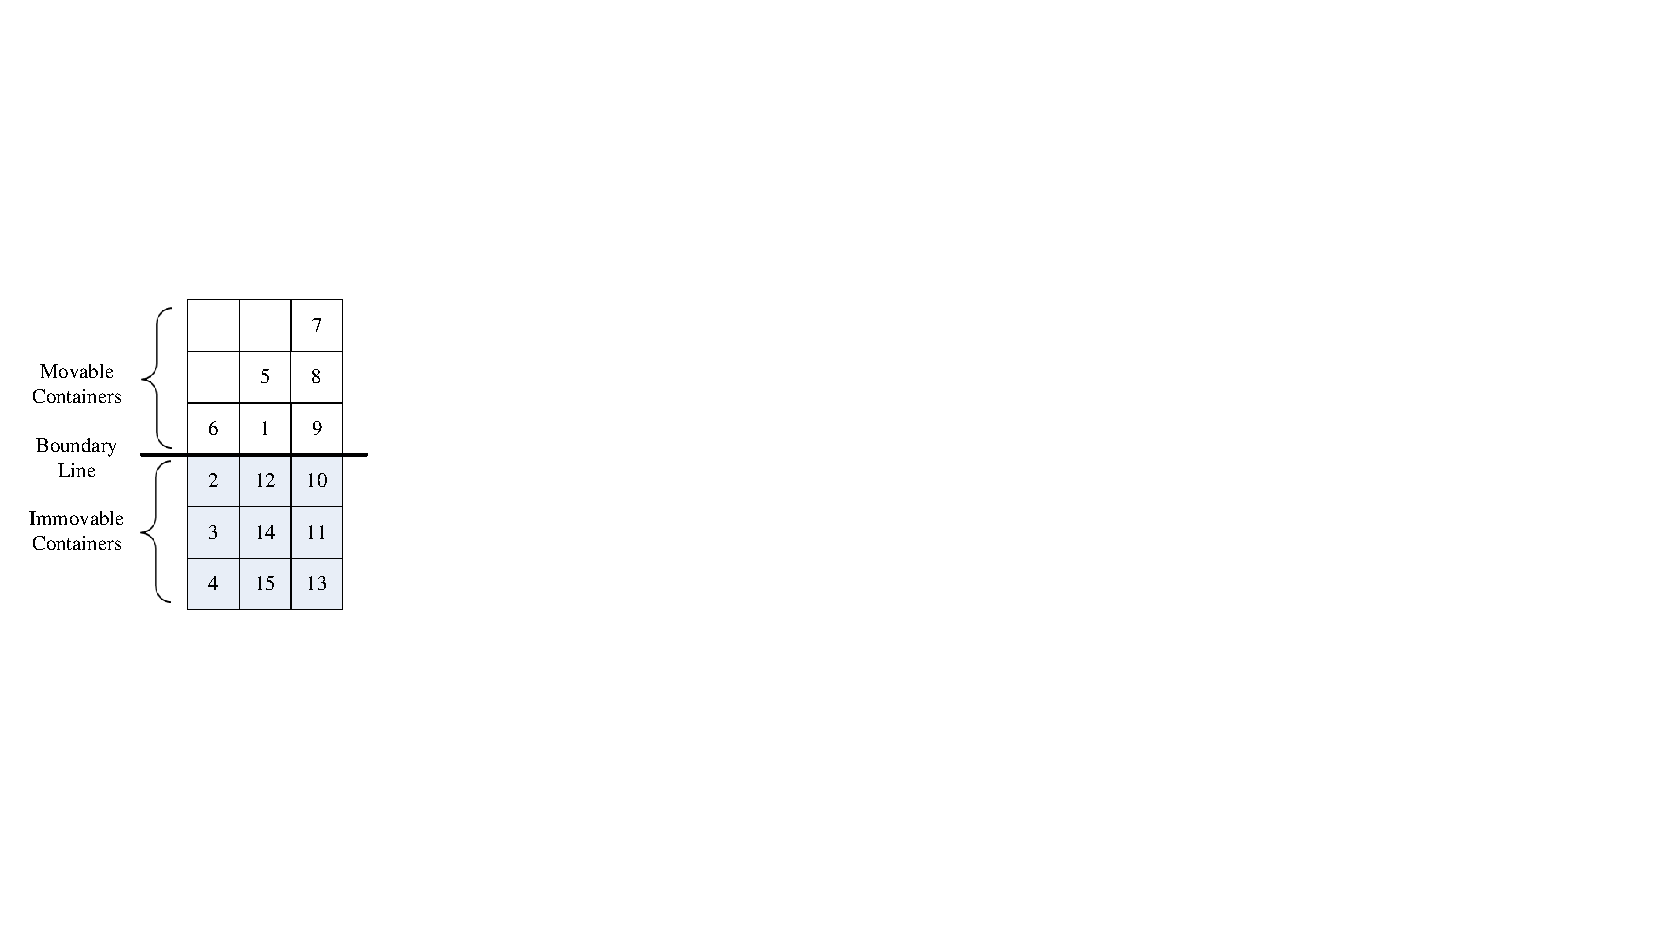
\includegraphics{fig4_1.pdf}}}
\subfigure[Case 2]{
    \label{fig10:2}
    \resizebox{0.3 \textwidth}{!}{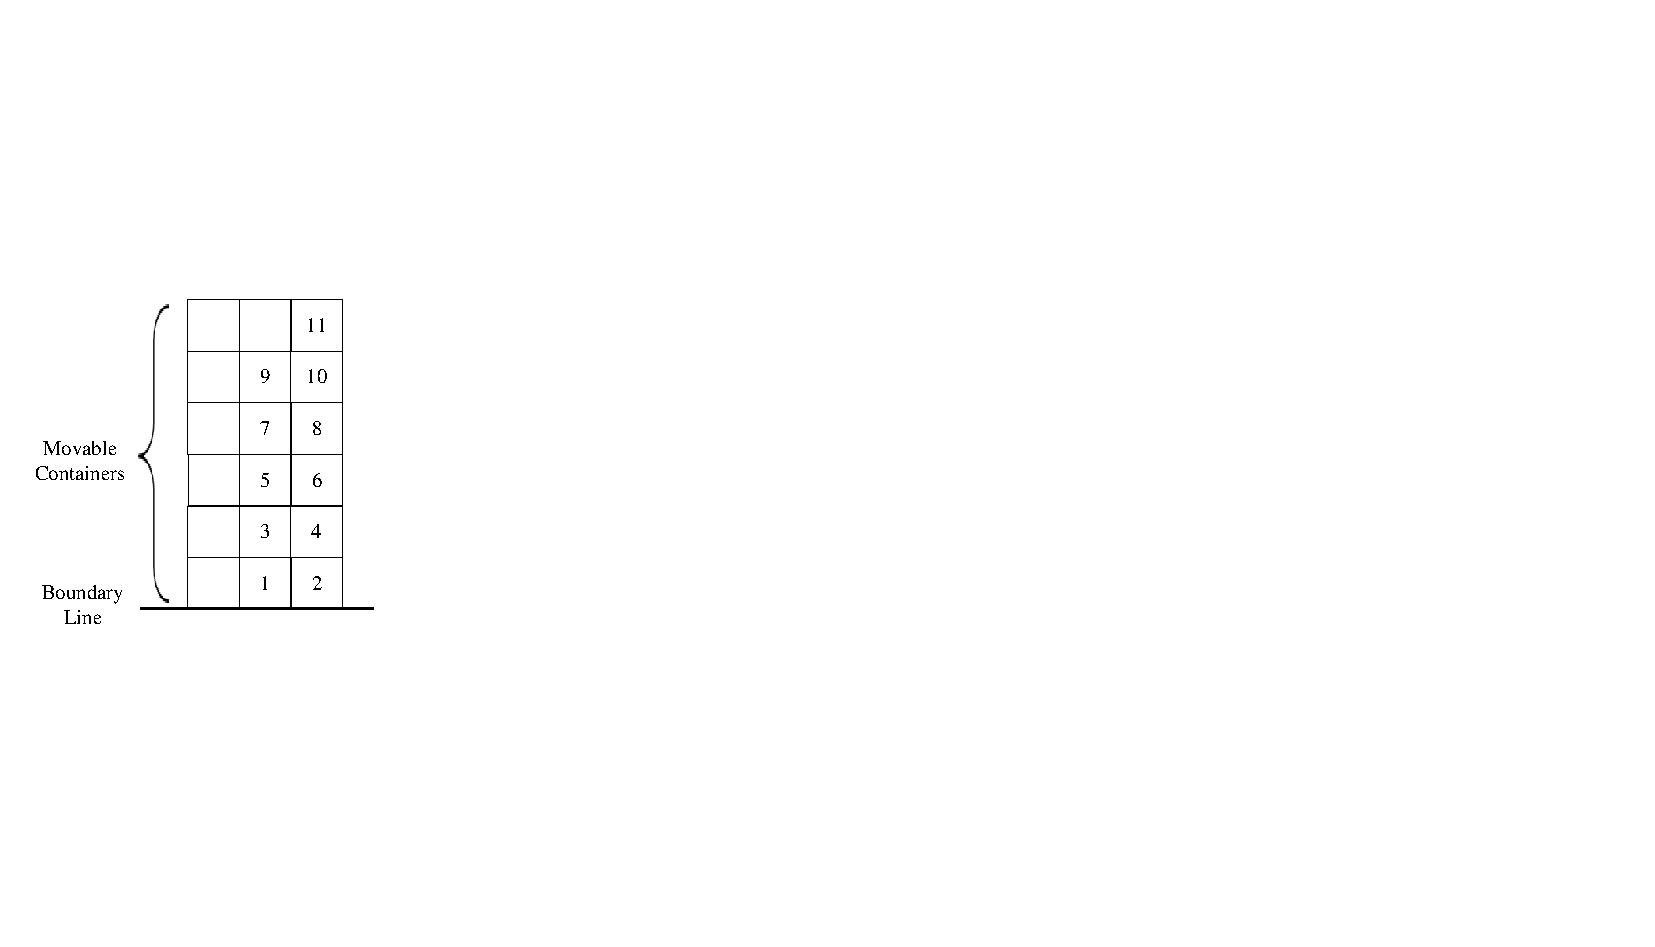
\includegraphics{fig4_2.pdf}}}
\caption{Boundary Line}
\label{fig4}
\end{figure}


\subsection{Feasibility check}

The feasibility of any CPMP/CPMPDS instance depends on the existence of a solution (movement sequence) that can transform the initial layout to a feasible layout.

\subsubsection{CPMP instances}

For any CPMP instance with $S=2$, a dirty layout is feasible if and only if: one stack $s_1$ is dirty, and the other stack $s_2$ is clean.
Stack $s_1$ has two parts: the lower part and the higher part, where containers have a non-increasing order and non-decreasing order of group labels from bottom to up, respectively.
In addition, the size of the higher part must be no larger than $e(s_2)$, and stack $s_2$ can accommodate the topmost container of stack $s_1$.

For any CPMP instance with $S\ge3$, all movable containers can be rearranged in any order based on Theorem \ref{the:1}.
The instance is concluded to be feasible if all stacks have no immovable containers.
Otherwise, all movable containers are removed to determine if they can be piled on the left immovable containers, which results in a clean layout regardless of the specific movement sequence. $G$-dimensional vectors $\mathbf S$ and $\mathbf D$ are introduced to this end to record slot supply and demand above the boundary line, respectively.
Initially, all elements of $\mathbf S$ and $\mathbf D$ are zero. For each stack $s$, $H-\id{im}$ is added to element $\mathbf S_g$ if the group label of its topmost immovable container is $g$.
The notation $\id{im}$ from Lemma \ref{lem:1} is the number of immovable containers in a stack. Element $\mathbf D_g$ of $\mathbf D$ records the number of movable containers with group label $g$.

An instance is feasible if and only if the demand of each group does not exceed the supply of the corresponding group, namely, $\mathbf S_g+\sum\limits_{i>g}\mathbf S_i-\sum\limits_{i>g}\mathbf D_i\ge \mathbf D_g$.
In another word, an instance is feasible if and only if the surplus for each group is non-negative, i.e.,
\begin{equation}
\label{equ:2}
\sum\limits_{i\ge g}\mathbf S_i-\sum\limits_{i\ge g}\mathbf D_i\ge0, \quad g=1,\dots,G
\end{equation}

\subsubsection{CPMPDS instances}

Any CPMPDS instance with $S=2$ is feasible if and only if the initial layout is feasible. Let stack $s_2$ be the dummy stack and stack $s_1$ be the other stack. A noteworthy case is that containers are piled in a non-decreasing order of group labels from bottom to up in stack $s_1$, and stack $s_2$ is empty. Although all containers can be relocated to stack $s_2$ one by one, which results in a clean layout with stack $s_1$ empty, the case is still infeasible in our opinion because stack $s_2$ should be empty in the final layout. This condition cannot be changed in any way, because the position of trucks cannot change.

All CPMPDS instances with $S\ge3$ are feasible. The number of immovable containers $\id{im}=0$, because an empty dummy stack exists. All containers can be rearranged in any order.
%Then they must can be rearranged in an order where all containers within a stack are piled in a decreasing order of group labels from the bottom up which is a feasible final layout.
Thus, any CPMPDS instance with $S\ge3$ is feasible.

\subsection{Lower bound}

In this section, a new method is proposed to calculate the lower bound of the number of movements necessary to reach a clean layout. The calculation of the lower bound of the CPMP is demonstrated. The lower bound of the CPMPDS requires only a small modification on the lower bound of the CPMP.

\subsubsection{Lower bound for the CPMP}

The lower bound is obtained by estimating the number of movements that belong to different movement types.
\begin{enumerate}
\setcounter{enumi}{0}
\item Dirty--Clean movements
\end{enumerate}

The number of dirty containers in a given layout is $\sum_{s=1}^S d(s)$. Each dirty container requires at least one movement to become clean; thus, the lower bound of the number of Dirty--Clean movements is $\id{num}_\id{DC}=\sum_{s=1}^S d(s)$.

\begin{enumerate}
\setcounter{enumi}{1}
\item Dirty--Dirty movements
\end{enumerate}

If all stacks are dirty in a layout, at least one stack should become clean to accommodate containers. This step is done by moving dirty containers of a stack to other dirty stacks. The least number of such Dirty--Dirty movements is $\id{num}_\id{DD} = \min\limits_{s=1, \dots, S} d(s)$.

\begin{enumerate}
\setcounter{enumi}{2}
\item Clean--X movements
\end{enumerate}

Before proceeding to explain the calculation, the concept of skyline is first introduced. A skyline is any vertical partition that separates a layout into higher and lower parts, where the lower part must be clean. The bold line in Figure \ref{fig5} is an example of a skyline. The boundary line in Figure \ref{fig4} is a special skyline that separates immovable and movable containers. A skyline can be represented by a vector $\id{SL}$ such that each element $\id{SL}_s$ represents the skyline segment across stack $s$. Segment $\id{SL}_s$ is described by the container underneath; the tier and group numbers of $\id{SL}_s$ are equal to those of the associated container. For example, in Figure \ref{fig5}, $\id{tn}(\id{SL}_{2})=3$ and $g(\id{SL}_{2})=1$.


\begin{figure*}[htbp]
\centering
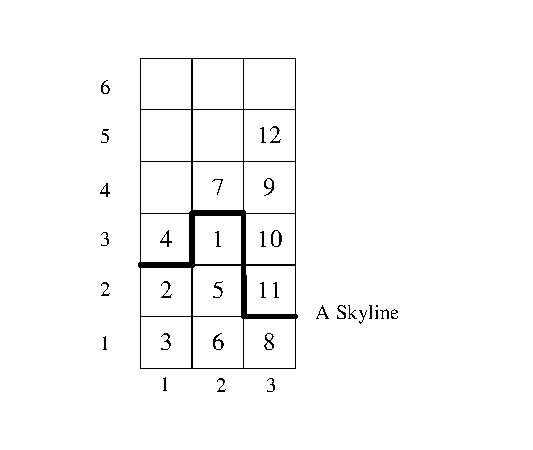
\includegraphics[width=0.3\textwidth]{fig5.pdf}
\caption{A skyline}
\label{fig5}
\end{figure*}

Supply and demand vectors, denoted as $\mathbf S^\id{SL}$ and $\mathbf D^\id{SL}$, record the numbers of slots and containers above \id{SL}. The $g$-th element of $\mathbf S^\id{SL}$ is $\mathbf S^\id{SL}_g=\sum\limits_{s:g(\id{SL}_s)=g}H-\id{tn}(\id{SL}_s)$, while the $g$-th element of $\mathbf D^\id{SL}$ is the number of containers above $\id{SL}$ with group label $g$.

For ease of explanation, Clean--Dirty and Clean--Clean movements are merged as Clean--X movements. The number of moved clean containers is a lower bound of the number of Clean--X movements. Ideally, pre-marshalling work involves dirty containers only and leaves clean containers unmoved. In some cases, however, achieving a clean layout is impossible without moving clean containers. The number of clean containers that need to be moved can be counted by the following process: given a bay, all dirty containers and a set of clean containers $C$ are removed from the layout, then slots are reassigned to removed containers. The resultant layout is required to be clean. Removed containers within a stack should be consecutive, i.e., if two containers from the same stack are removed, containers between them are also removed. The size of smallest $C$ is the number of Clean--X movements $\id{num}_{CX}$. Finding the smallest $C$ is equivalent to finding the skyline with the fewest clean containers in its higher part (smallest skyline) as well as non-negative surpluses (Equation \ref{equ:3}).

\begin{equation}
\label{equ:3}
\sum\limits_{i\ge g}\mathbf S^\id{SL}_i-\sum\limits_{i\ge g}\mathbf D^\id{SL}_i\ge0, \quad g=1,\dots,G
\end{equation}

To find the smallest skyline, a basic skyline $\id{SL}$ that separates clean and dirty containers is drawn. Next a depth-first-search (DFS) is deployed to push a certain segment of $\id{SL}$ one tier down in each branching. The leaves of the search tree are all the skylines with non-negative surpluses; the one with the fewest pushes is selected and the number of pushes is $\id{num}_\id{CX}$.

To conclude, the lower bound can be defined as $\id{LB}_\id{DFS}=\id{num}_\id{DC}+\id{num}_\id{DD}+\id{num}_\id{CX}$.

\subsubsection{Clean--X movements by maximum knapsack}

The lower bound $\id{LB}_\id{DFS}$ is time-consuming because a DFS is used to calculate $\id{num}_{\id{CX}}$. A maximum knapsack method (MKM) is proposed to approximate $\id{num}_{CX}$. A basic skyline SL that separates clean and dirty containers is drawn, then the smallest skyline with non-negative surplus for a single group is obtained instead of for all groups. This search is repeated for each group, and the maximum skyline is selected amongst all obtained skylines.

For a given group label $g$, a knapsack-like problem is solved to find the smallest skyline with non-negative surplus in terms of $g$. Stacks in the bay are regarded as items, where each item $s\in\{1,\dots,S\}$ has value $v_s$ and cost $c_s$. The objective is to select a set of items with the lowest cost such that the total value selected is at least $V$. Every item can only be selected at most once. $c_s$ is the number of clean containers in stack $s$ to be moved to accommodate group $g$, while $v_s$ is the resultant number of slots available for group $g$, i.e., $v_s=c_s+e(s)$. $V$ is the number of dirty containers with group label $g(c)\ge g$. The decision variable $x_s$ is 1 if stack $s$ is selected; otherwise, $x_s=0$. The integer programming model of this knapsack-like problem is show in Equation \ref{equ:4} and can be easily solved by dynamic programming.


\begin{equation}
\label{equ:4}
\begin{array}{rl}
\min & \sum\limits_{s=1}^S c_s x_s\\
\mathrm{s.t.} &\sum\limits_{s=1}^S v_s x_s\ge V\\
&x_s\in\{0,1\}, \quad s=1,\dots,S
\end{array}
\end{equation}

MKM is not as precise as DFS, but the solution gap is quite small and the computation speed is improved. The lower bound provided by MKM is denoted as $\id{LB}_{\id{MKM}}$.

\subsubsection{Comparison with existing lower bound}
The current state-of-the-art lower bound $\id{LB}_\id{BF}$ was proposed by \cite{BF2012}, which also consists of three parts: Dirty--Clean, Dirty--Dirty and Clean--X movements.
The first two types are calculated in the same manner as $\id{LB}_\id{DFS}$ and $\id{LB}_\id{MKM}$ in this paper. For Clean--X movements, a basic skyline SL that separates clean and dirty containers is drawn, then they only take the group label $g^*$ with the smallest surplus $\id{min}=\min\limits_g\sum\limits_{i\ge g}\mathbf S^\id{SL}_i-\sum\limits_{i\ge g}\mathbf D^\id{SL}_i$. If $\id{min}$ is negative, $\sum\limits_{i\ge g^*}\mathbf D^\id{SL}_i$ surpasses $\sum\limits_{i\ge g^*}\mathbf S^\id{SL}_i$ by $|\id{min}|$, which means that clean containers need to be moved to accommodate these $|\id{min}|$ dirty containers. The number of moved clean containers $\id{num}_\id{CX}$ is estimated by \cite{BF2012} as follows: suppose one stack is able to (although in fact it may not be able to) accommodate $H$ dirty containers with $g\ge g^*$, then $|\id{min}|$ dirty containers need at least $\left\lceil\frac{|\id{min}|}{H}\right\rceil$ stacks. As slots supply of stacks with $g(\id{SL}_s)\ge g^*$ have been calculated into $\sum\limits_{i\ge g^*}\mathbf S^\id{SL}_i$, only stacks with $g(\id{SL}_s)< g^*$ (denote as set \id{AS}) can provide slots for $|\id{min}|$ dirty containers. Suppose $c_s$ is the number of clean containers in stack $s$ to be moved to accommodate group $g^*$, sort $c_s$ of stacks in set $\id{AS}$ ascendingly. The first $\left\lceil\frac{|\id{min}|}{H}\right\rceil$ stacks are selected and $\id{num}_\id{CX}=\sum\limits_{s=1}^{s=\left\lceil\frac{|\id{min}|}{H}\right\rceil}c_s$.

From the mathematical perspective, the method of \cite{BF2012} is equivalent to solve the following model, stacks in the bay are regarded as items, where each item $s\in\{1,\dots,S\}$ has value $v_s'$ and cost $c_s$. The objective is to select a set of items with the lowest cost such that the total value selected is at least $V$. Every item can only be selected at most once. $c_s$ is the number of clean containers in stack $s$ to be moved to accommodate group $g^*$, while $v_s'$ is the resultant number of slots available for group $g^*$. According to \cite{BF2012} $v_s'=H$ if $g(\id{SL}_s)<g^*$, otherwise $v_s'=c_s+e(s)$. $V$ is the number of dirty containers with group label $g(c)\ge g^*$. The decision variable $x_s$ is 1 if stack $s$ is selected; otherwise, $x_s=0$. The integer programming model is show in Equation \ref{equ:5}.


\begin{equation}
\label{equ:5}
\begin{array}{rl}
\min & \sum\limits_{s=1}^S c_s x_s\\
\mathrm{s.t.} &\sum\limits_{s=1}^S v_s' x_s\ge V\\
&x_s\in\{0,1\}, \quad s=1,\dots,S
\end{array}
\end{equation}

Compare Model \ref{equ:4} with Model \ref{equ:5}, all parameters are the same except for $v_s$ ($v_s'$). The solution to Model \ref{equ:5} is the solution to Model \ref{equ:4}, while the reverse does not stand. The solution space of Model \ref{equ:5} is larger than Model \ref{equ:4}, thus the optimal solution to Model \ref{equ:4} is no smaller than that to Model \ref{equ:5}. Furthermore, \cite{BF2012} only solve Model \ref{equ:5} once for $g^*$, whereas this paper solves Model \ref{equ:4} for every group and then take the maximal result as $\id{num}_\id{CX}$. As a result, the lower bound $\id{LB}_\id{MKM}$ dominates $\id{LB}_\id{BF}$: $\id{LB}_\id{BF}\le \id{LB}_\id{MKM}\le \id{LB}_\id{DFS}$.
\subsubsection{Lower bound of the CPMPDS}

The lower bound of the CPMPDS consists of three parts: Dirty--Clean, Dirty--Dirty, and Clean--X movements.

The lower bound of Dirty--Clean movements is equal to the number of dirty containers. For Dirty--Dirty movements $\id{num}_\id{DD}=\min\limits_{s\neq s_d} d(s)$, where $s_d$ is the dummy stack. If all stacks except for the dummy stack are dirty, then dirty containers from at lest one stack need to be relocated to other dirty stacks or the dummy stack. In both situations, these containers are still dirty after relocation.

The lower bound of Clean--X movements is the number of clean containers moved to make all containers clean and dummy stack empty, which is equivalent to assigning containers only to the first $S-1$ stacks and ignoring the dummy stack.

Based on the analysis above, $\id{LB}_\id{DFS}$ ($\id{LB}_\id{MKM}$) of a CPMPDS instance is equal to $\id{LB}_\id{DFS}$ ($\id{LB}_\id{MKM}$) of the corresponding CPMP instance with the dummy stack removed.

\section{Target guided heuristic}
\label{sec:heu}

In this section, we present a target guided heuristic (TGH) for the CPMP/CPMPDS. This heuristic can be used as an independent algorithm, as well as a component of more complex algorithms in the next section.

The main idea of the heuristic is: starting from the largest priority label, fix one container in a certain slot each time. After a container is fixed, it will not be relocated any more, except a special case. We resolve the special case by relocating fixed containers back. This will be explained later.
As containers are fixed continuously, all the stacks become clean in the end. Hence, this heuristic guarantees to find a solution for any feasible instance. A complete description of the framework is displayed in Algorithm \ref{alg:heu}.
%It suits both the CPMP and the CPMPDS.

\begin{algorithm}[htbp]
	\caption{The target guided heuristic for the CPMP/CPMPDS}
	\label{alg:heu}
	\begin{codebox}
	\Procname{\proc{TGH (\id{inilay})}}
	\li $\id{curlay} = \id{inilay}$
    \li mark all the immovable containers in \id{curlay} as fixed
    \li mark all the movable containers in \id{curlay} as unfixed
    \li $\id{g} = G$
    \li \While ($g\neq0$)
    \li \Do
            mark the clean containers with group label \id{g} as fixed\label{heu:c}
    \li     \id{conList} = the set of candidate containers
    \li     \While($\id{conList} \neq \emptyset$)\label{heu:l}
    \li     \Do
                \id{stkList} = the set of candidate stacks
    \li         select the target container and the target stack from \id{conList} and \id{stkList}, respectively
    \li         apply a giant move to fix the target container to the target stack
            \End
    \li $g=g-1$
        \End
%	\li \Return;
	\end{codebox}	
\end{algorithm}

%The heuristic starts with the initial layout $\id{inilay}$. In the initialization stage, all the immovable containers are labeled as fixed while movable containers as unfixed.
%The current layout $\id{curlay}$ is initialized with $\id{inilay}$ and current group $g$ is initialized with $G$. In the following, the algorithm fixes containers one by one according to a descending order of group numbers.
%When fixing containers with a certain group label, clean containers are fixed in their original positions directly and marked as fixed (Line \ref{heu:c}).
%For the dirty containers, we fix them successively. In the current layout, we select one target container and one target stack, and apply several movements so as to fix the target container to the target stack, resulting a new layout. Such a process is called one transition.
In Algorithm \ref{alg:heu}, a movement sequence which fixes a target container to a target stack is named as a \textbf{giant move}. In contract, one movement operation is coined as a \textbf{baby move}.

The advantage of our heuristic is that containers are fixed one by one, therefore it is very easy to customize the heuristic for other CPMP variants, for example, variants which require the containers in a final layout adhere to special distribution characteristics. It only needs to modify the rules of candidate stacks selection, making the containers fixed according to the required distribution.



\subsection{Candidate containers and stacks selection}
\label{sec:can}
When processing group $g$, the set of candidate containers is comprised of all the unfixed containers with group label $g$. Candidate stacks are selected based on the candidate containers.
To be a candidate stack, a stack must be able to accommodate group $g$ after relocating some of its containers.
%For example, in Figure \ref{fig4:1}, the available stack for container 6 is only the stack in the middle.
In the CPMPDS, the dummy stack cannot be a candidate stack. Among all the available stacks, we prefer stacks which can accommodate $g$ without any relocation. If there does not exist such a stack, we select an available stack randomly.

\subsection{Target pair selection}
\label{sec:tar}
An evaluation scheme is designed to evaluate the attractiveness of fixing a candidate container to a candidate stack.
%The candidate containers are from \id{conList}, and the candidate stacks are the result from procedure \proc{CandidateStack}.
%The attractiveness of each candidate pair $(c,s)$ is evaluated by an evaluation scheme and the most attractive pair is selected as the target container \id{con} and target stack \id{stk}, respectively.
Intuitively, we want the movements as few as possible. A function $f(c,s)$ is introduced to roughly estimate the movement cost for fixing container $c$ to stack $s$. If container $c$ is currently in stack $s$, $f(c,s)=\id{uf}(s)$; otherwise, $f(c,s)=\id{uf}(s)+o(c)$. Then we prefer to fix containers at lower tiers, i.e., stacks with smaller number of fixed containers $h(s)-\id{uf}(s)$ is preferred. This preference makes the fixed containers distributed evenly among stacks. In summary, 2-tuple $(f(c,s), h(s)-\id{uf}(s))$ evaluates the attractiveness.

When selecting the target pair, each container from candidate containers and each stack from candidate stacks make up of a candidate pair. Sort all the candidate pairs in the ascending lexicographical order of the evaluation values and the best one is selected as the target pair.

\subsection{A giant move}

Given the target container $c^*$ and the target stack $s^*$, a giant move is executed to fix container $c^*$ in stack $s^*$. The target slot of $s^*$ for $c^*$ is the slot just above the fixed containers of $s^*$. Hereafter, we do not explicitly point out the target slot.
A giant move does not disturb the positions of already fixed containers. According to whether the origin of container $c^*$ is stack $s^*$ or not, the giant move includes two cases. We describe the concrete movements for the two cases separately.

\subsubsection{Case 1: fixing to the same stack}

In Case 1, the origin of container $c^*$ is stack $s^*$. In the first step, all the containers above $c^*$ are relocated; container relocation strategy will be explained in Section \ref{sec:rel}. After that, container $c^*$ is at the top of stack $s^*$ and it needs a stack for temporary storage. We consider the highest non-full stacks for temporary storage. Among such stacks, a dirty stack is preferred. Denote the temporary stack as stack $\id{ts}$.

Before moving container $c^*$ to stack $\id{ts}$, we observe in advance where to relocate the unfixed containers under $c^*$ so that stack $s^*$ can accommodate $c^*$. Avoiding occupying stack $\id{ts}$ and $s^*$ is a straightforward idea. On top of this, denote the set of stacks except stack $\id{ts}$ and $s^*$ as $\id{AS}$, compute its available empty slots $\id{nslot} = \sum\limits_{s\neq s^*, \id{ts}}e(s)$, and compare $\id{nslot}$ with $\id{uf}(s^*)$. According to the comparison results, three scenarios are raised.

\begin{enumerate}
\setcounter{enumi}{0}
\item $\id{nslot}\ge \id{uf}(s^*)-1$
\end{enumerate}
In this scenario, the empty slots of $\id{AS}$ are enough to store the unfixed containers under $c^*$. We move $c^*$ directly to stack $\id{ts}$ and then relocate all the unfixed containers under $c^*$ to the empty slots of $\id{AS}$. At last, $c^*$ is moved back to stack $s^*$.

\begin{enumerate}
\setcounter{enumi}{1}
\item $0<\id{nslot}< \id{uf}(s^*)-1$
\end{enumerate}
In this scenario, the empty slots of $\id{AS}$ are not enough for the unfixed containers under $c^*$. Following moving $c^*$ to stack $\id{ts}$, only the first $\id{nslot}-1$ unfixed containers under $c^*$ are relocated to the empty slots of $\id{AS}$, with an empty slot left. We occupy the last empty slot by moving $c^*$ to it. Then the remained unfixed containers in stack $s^*$ are relocated to stack $\id{ts}$. At last, $c^*$ is moved back to stack $s^*$.
\begin{enumerate}
\setcounter{enumi}{2}
\item $\id{nslot}=0$
\end{enumerate}
In this scenario, all the stacks belonging to $\id{AS}$ are full. We cannot move $c^*$ directly to stack $\id{ts}$ otherwise it will be buried soon by the unfixed containers in stack $s^*$. A top slot is needed to temporarily store $c^*$. To create such an empty slot, we seek a top container from all the top containers of stacks belonging to $AS$. The top container $c$ is selected as follows.

If stack \id{ts} is a clean stack, the preference is:
\begin{enumerate}[1.]
\item Among dirty containers which stack \id{ts} can accommodate, select the one with the largest group label;
\item Among clean containers which stack \id{ts} can accommodate, select the one with the largest group label;
\item The dirty container with the smallest group label;
\item The clean container with the smallest group label.
\end{enumerate}

If stack \id{ts} is a dirty stack, the preference is:
\begin{enumerate}[1.]
\item The dirty container with the smallest group label;
\item The clean container with the smallest group label.
\end{enumerate}
After container $c$ is moved to stack $\id{ts}$, its origin is occupied by $c^*$. In the following, all the unfixed containers of stack $s^*$ are relocated to stack $\id{ts}$. At last, $c^*$ is moved to stack $s^*$. If $c$ is a fixed container, we should restore it to its origin. Suppose the origin of $c$ is stack $\id{cs}$, relocate all the containers above $c$ and move $c$ back to stack $\id{cs}$.
%\begin{algorithm}[htbp]
%	\caption{Fix the target container to the same stack}
%	\label{alg:fixs}
%	\begin{codebox}
%	\Procname{\proc{FixS(\id{con}, \id{curlay})}}
%    \li $\id{os}=\id{sn}(\id{con})$ and \id{g} = $g(\id{con})$;
%    \li \id{curlay} = \proc{Move\_Containers($O(\id{con})$, \id{g}, $-1$)};
%    \li \id{ts} = select a non-full stack with the highest height, and prefer a dirty stack among such stacks;
%    \li \id{nslot} = $\sum_{s\neq \id{os},\id{ts}}e(s,\id{curlay})$;
%    \li \If ($\id{nslot}\ge \id{uf}(\id{os}, \id{curlay})-1$)
%    \li     \Then
%            Put \id{con} to the top of stack \id{ts} and update \id{curlay};
%    \li     \id{curlay} = \proc{Move\_Containers($\id{uf}(\id{os},\id{curlay})$, \id{g}, \id{ts})};
%    \li     Put \id{con} to the top of stack \id{os} and update \id{curlay};
%    \li \ElseIf ($\id{nslot}>0$)
%    \li     \Then
%            Put \id{con} to the top of stack \id{ts} and update \id{curlay};
%    \li     \id{C} = set of the top $nslot-1$ containers of stack \id{os};
%    \li     \id{curlay} = \proc{Move\_Containers(\id{C}, \id{g}, \id{ts})};
%    \li     Put \id{con} to $S\backslash \{\id{os}, \id{ts}$\} and update \id{curlay};{\color{red}what does this line mean?}
%    \li     \id{curlay} = \proc{Move\_Containers($\id{uf}(\id{os}, \id{curlay})$, \id{g}, $-1$)};
%    \li     Put \id{con} to the top of stack \id{os} and update \id{curlay};
%    \li \Else
%    \li     \id{ts2} = select a full stack with parameter \id{ts} according to rule R;\label{fixs:r}
%    \li     \id{c^*} = the top container of stack \id{ts2};
%    \li     Put \id{c^*} to stack \id{ts}, put \id{con} to stack \id{ts2}, and update \id{curlay};
%    \li     \id{curlay} = \proc{Move\_Containers($\id{uf}(\id{os}, \id{curlay})$, \id{g}, $-1$)};
%    \li     Put \id{con} to the top of stack \id{os} and update \id{curlay};
%    \li     \If(\id{c^*} was fixed)\label{fixs:ms}
%    \li         \Then
%                \id{curlay} = \proc{Move\_Containers($O(c^*)$, \id{g}, \id{ts2})};
%    \li         Put \id{c^*} to stack \id{ts2} and update \id{curlay};\label{fixs:me}
%            \End
%        \End
%    \li \Return \id{curlay};
%	\end{codebox}	
%\end{algorithm}
\subsubsection{Case 2: fixing to a different stack}
In Case 2, the origin of container $c^*$ is not stack $s^*$. If $c^*$ is the topmost container and all the containers in stack $s^*$ are fixed containers, move $c^*$ to stack $s^*$ directly. If not, in spirit of Case 1, we define $\id{AS}$ as the set of all the stacks except stack $s^*$ and $\id{sn}(c^*)$ (the origin of $c^*$) and compare least movements required $f(c^*,s^*)$ with available slots $\id{nslot}=\sum\limits_{s\neq s^*,\id{sn}(c^*)}e(s)$. According to the comparison results, four scenarios are raised.
\begin{enumerate}
\setcounter{enumi}{0}
\item $\id{nslot}\ge f(c^*,s^*)$
\end{enumerate}
In this scenario, relocate all the containers above $c^*$ and unfixed containers in stack $s^*$ to the empty slots of $\id{AS}$. When relocation, each time we relocate the top container from stack $s^*$ or $\id{sn}(c^*)$ which has a larger group label. After that, container $c^*$ is moved to stack $s^*$.

\begin{enumerate}
\setcounter{enumi}{1}
\item $o(c^*)+1\le\id{nslot}< f(c^*,s^*)$
\end{enumerate}
In this scenario, containers above $c^*$ and the unfixed containers in stack $s^*$ cannot be relocated to the empty slots of $\id{AS}$ one-off. We choose to relocate all the containers above $c^*$ together with a subset of unfixed containers in stack $s^*$, with a total of $\id{nslot}-1$ containers, leaving one empty slot for $c^*$. Again, when relocation, select the topmost one with a larger group label each time. After relocating aforesaid containers, move $c^*$ to the unique empty slot left in $\id{AS}$. In the following, relocate the remaining unfixed containers in stack $s^*$ to stack $\id{sn}(c^*)$. At last, container $c^*$ is moved to stack $s^*$.

\begin{enumerate}
\setcounter{enumi}{2}
\item $1\le\id{nslot}< o(c^*)+1$
\end{enumerate}
In this scenario, we only relocate $\id{snlot}-1$ containers of stack $\id{sn}(c^*)$ to the empty slots of $\id{AS}$, and then relocate remaining containers above $c^*$ to stack $s^*$. At present, $c^*$ is on the top and moved to the unique empty slot in $AS$. Then all the unfixed containers in stack $s^*$ including those originated from stack $\id{sn}(c^*)$ are relocated to stack $\id{sn}(c^*)$. At last, container $c^*$ is moved to stack $s^*$.

\begin{enumerate}
\setcounter{enumi}{3}
\item $\id{nslot}=0$
\end{enumerate}
In this scenario, it is somehow like the third scenario in Case 1. We need to create an empty slot for $c^*$ for temporary storage. The selection of a top container from a full stack is the same with that mentioned in Scenario 3 of Case 1. Denote the selected top container as $c$ and its origin as stack $\id{cs}$. We first move $c$ to stack $s^*$, and relocate all the containers above $c^*$ to stack $s^*$. Then move $c^*$ to stack $\id{cs}$ for temporary storage. Next, all the unfixed containers of stack $s^*$ including $c$ are relocated to stack $\id{sn}(c^*)$. At last, $c^*$ is moved to stack $s^*$. Similar to the issue raised in Scenario 3 of Case 1, container $c$ may be a fixed container. If that is the case, we also have to restore $c$ to stack $\id{cs}$.


%\begin{algorithm}[htbp]
%	\caption{Fix the target container to a different stack}
%	\label{alg:fixd}
%	\begin{codebox}
%	\Procname{\proc{FixD(\id{con}, \id{stk}, \id{curlay})}}
%    \li \If ($f(\id{con}, \id{stk})=0$)
%    \li \Then
%        Put \id{con} to \id{stk} directly and return the updated \id{curlay};
%        \End
%    \li $\id{os} = \id{sn}(\id{con})$ and $\id{g}=g(\id{con})$;
%    \li \id{nslot} = $\sum_{s\neq \id{os},\id{stk}}e(s,\id{curlay})$;{\color{red}what is ts here?}
%    \li \If ($\id{nslot}\ge f(\id{con},\id{stk})$)
%    \li     \Then
%            \id{curlay} = \proc{Move\_Containers($\id{uf}(\id{stk},\id{curlay})\&O(\id{con})$, \id{g}, $-1$)};
%    \li     Put \id{con} to the top of stack \id{stk} and update \id{curlay};
%    \li \ElseIf ($O(\id{con})\le \id{nslot}-1$)
%    \li     \Then
%            \id{num} = $\id{nslot}-1-O(\id{con})$;
%    \li     \id{C} = top \id{num} containers of stack \id{stk};
%    \li     \id{curlay} = \proc{Move\_Containers($C\&O(\id{con})$, \id{g}, $-1$)};
%    \li     Put \id{con} to $S\backslash \{\id{os}, \id{stk}$\} and update \id{curlay};{\color{red}what is $S\backslash \{\id{os}, \id{stk}$\}?}
%    \li     \id{curlay} = \proc{Move\_Containers($\id{uf}(\id{stk}, \id{curlay})$, \id{g}, $-1$)};
%    \li     Put \id{con} to the top of stack \id{stk} and update \id{curlay};
%    \li \ElseIf ($\id{nslot}-1\ge0$)
%    \li     \Then
%                \id{C} = top $\id{nslot}-1$ containers of stack \id{os};
%    \li         \id{curlay} = \proc{Move\_Containers(\id{C}, \id{g}, \id{stk})};
%    \li     Put all the containers in $O(\id{con})$ to \id{stk} and update \id{curlay};
%    \li     Put \id{con} to $S\backslash \{\id{os}, \id{stk}\}$ and update \id{curlay};{\color{red}what does this line mean?}
%    \li     \id{curlay} = \proc{Move\_Containers($\id{uf}(\id{stk}, \id{curlay})$, \id{g}, $-1$)};
%    \li     Put \id{con} to the top of stack \id{stk};
%    \li \Else
%    \li     \id{ts} = select a full stack with parameter \id{stk} according to rule R;\label{fixd:r}
%    \li     \id{c^*} = top container of stack \id{ts};
%    \li     Put \id{c^*} to stack \id{stk} and update \id{curlay};
%    \li     Put all containers in $O(\id{con})$ to stack \id{stk} and update \id{curlay};
%    \li     Put \id{con} to stack \id{ts} and update \id{curlay};
%    \li     \id{curlay} = \proc{Move\_Containers($\id{uf}(\id{stk},\id{curlay})\&c^*$, \id{g}, $-1$)};
%    \li     Put \id{con} to stack \id{stk} and update \id{curlay};
%    \li     \If(\id{c^*} was fixed)\label{fixd:ms}
%    \li         \Then
%                \id{curlay} = \proc{Move\_Containers($O(c^*)$, \id{g}, \id{ts})};
%    \li         Put \id{c^*} to \id{ts} and update \id{curlay};\label{fixd:me}
%            \End
%        \End
%    \li \Return \id{curlay};
%	\end{codebox}	
%\end{algorithm}


\subsection{Container relocation}
\label{sec:rel}
%Procedure \proc{Move\_Containers} is described in Algorithm \ref{alg:mc}. It moves a set of containers from their current positions.
%\id{g} is the group label of current target container in Algorithm \ref{alg:heu} and \id{tubas} is forbidden to be the destination stack of \id{C}. Every time, a top container \id{c} is moved.
%If \id{C} includes two top containers from two stacks, then \id{c} is the one with larger group label. The procedure \proc{Select\_Stack\_For} returns the destination stack for container \id{c}.
%But if the found destination stack \id{s} can be fulfilled (procedure \proc{Fulfill}), then \proc{Select\_Stack\_For} loops until a destination stack which can not be fulfilled is found. At last, the container \id{c} is put to the stack \id{s}.

%\begin{algorithm}[htbp]
%	\caption{Move a set of containers from their current positions}
%	\label{alg:mc}
%	\begin{codebox}
%	\Procname{\proc{Move\_Containers(\id{C}, \id{g}, \id{tabus})}}
%    \li \While ($C$ is not empty)
%    \li \Do
%            \If \id{C} includes containers from two stacks
%    \li     \Then
%            \id{c} = the container with a larger group label between the top containers of two stacks;
%    \li     \Else
%            \id{c} = the topmost container among C;
%            \End
%    \li     Remove \id{c} from \id{C};
%    \li     \id{s} = \proc{Select\_Stack\_For(\id{c}, \id{g}, \id{tabus})};
%    \li     \While (\proc{Fulfill(\id{s}, \id{c})})
%    \li     \Do
%                \id{s} = \proc{Select\_Stack\_For(\id{c}, \id{g}, \id{tabus})};
%            \End
%    \li     Put \id{c} to the top of \id{s};
%        \End
%	\end{codebox}	
%\end{algorithm}
Container relocation occurs when a container blocks the target container or it is an unfixed container in the target stack. Generally speaking, we can relocate a container $c$ to any stack, excluding prohibited stacks such as the target stack, the origin of the target container, and sometimes the temporary stack for the target container. Whereas we would like $c$ to be relocated at an appropriate stack, so that it will not block others or be blocked by others in the future. Suppose the target container in process is $c^*$. Apart from prohibited stacks and full stacks, we find the destination stack for relocating $c$ according to the following preference.
\begin{enumerate}[1.]
\item A clean stack which can accommodate \id{c}. If there are several such stacks, prefer the one whose top container has the smallest group label;

\item A dirty stack whose dirty container with the largest group label $\id{ldg}\le g(c)$. If there are several such stacks, prefer the one with the largest $\id{ldg}$;

\item A dirty stack whose dirty container with the largest group label $g(c)<\id{ldg}<g(c^*)$. If there are several such stacks, prefer the one with the smallest $\id{ldg}$;

\item A clean stack whose top container has the largest group label;

\item A dirty stacks whose dirty container with the largest group label $\id{ldg}=g(c^*)$.
\end{enumerate}

%With the assistance of stack preference, it can find suitable destination stacks for relocated containers. But one point can be improved.
When the selected destination can accommodate container $c$, we try \textbf{fulfillment} process. Denote the topmost container from the destination stack as $\id{dc}$. We are in hope of finding a top container $\id{fc}$ from a dirty stack whose group label falls in the range $g(c)<g(\id{fc})\le g(\id{dc})$.
If there is more than one top container satisfying such criterion, select the one with the largest group label and move it to the destination stack. As the layout changes after one time of fulfillment, we give up continuing relocating $c$ to the destination stack. Rather, we invoke the relocation procedure for $c$ again.
 %since $c$ may be relocated to another stack different from the destination stack.

The advantage of fulfillment is that slot space of clean stacks is fully utilized. This avoids the situation where a container with a small group label occupies the top of a stack, blocking the stack from accommodating dirty containers with larger group labels. Fulfillment is extremely efficient at the start of the heuristic when dirty containers with large group labels are quite many.

In our heuristic, every time the fulfillment is invoked, only one movement is carried out. After that the heuristic turns to relocate containers. This is different from that of \cite{Exposito2012} which carries out movements as many as possible in one fulfillment. We prefer to perform one movement each time because our intention is to relocate $c$ while fulfillment is only an auxiliary operation. Compared to a greedy fulfillment process, we are more eager to find whether a more suitable stack resulting from the fulfillment appears for relocating $c$. Performing fulfillment as much as possible, in the short run, deviates from our intention of relocating $c$. Moreover, over-fulfillment may cause the stacks fulfilled being emptied in later stages which brings more movements.

\subsection{Termination analysis}

Remind in Algorithm \ref{alg:heu}, we claim that our heuristic fixes containers one by one and therefore it guarantees to find a solution for any feasible instance. We do not mention the fact that a fixed container may be moved when fixing another container.
If that situation happens, we can not guarantee that the heuristic will terminate because it may fall into cycling. Fortunately we successfully deal with moved fixed containers. The only chance that a fixed container is moved when fixing other containers is in the situation $\id{nslot}=0$.
In other situations, all of the moved containers are unfixed ones. Once a fixed container is moved, we recover it back to its fixed position (the last scenarios of Case 1 and Case 2).
Undoubtedly, this recovery action brings more movements. But this avoids the heuristic cycling in vain and makes sure that the heuristic terminates.
Besides our work, all the other published work concerning the CPMP fail to guarantee algorithm termination theoretically.

\section{Beam search algorithms}
\label{sec:g2la}

Algorithm \ref{alg:heu} is just a greedy heuristic, in which the core idea is to fix containers one by one. In that heuristic, how to select target containers and stacks is completely based on the evaluation scheme.
Obviously, the precision of the scheme is very important; once it fails, the heuristic will be led to a wrong direction. To avoid this risk, we propose beam search algorithms in this section.

\subsection{Beam search with giant moves}

The first beam search algorithm maintains a beam of promising layouts and the number of such promising layouts in the beam is a user-defined parameter $\id{bw}$ (short for beam width). Initially, the beam only contains the initial layout. Then the beam search process extends the layouts in the beam iteratively by giant moves. Hence, we call the algorithm beam search with giant moves (BS-G).

For each layout $l$ in the beam, we perform a probing tree search with two parameters tree width $\id{tw}$ and tree depth $\id{td}$ to generate its children. Each child of $l$ is generated by selecting a container-stack pair and conducting a giant move. As the number of container-stack pairs is numerous, we select only a few of them. First only pairs with container part in the candidate container list and stack part in the candidate stack list are considered. The way in which candidate containers and stacks are produced is as mentioned in Section \ref{sec:can}. All of the candidate pairs are sorted based on the evaluation scheme values in Section \ref{sec:tar} and the first $\id{tw}$ pairs are selected; the corresponding giant moves are executed. To this end, we obtain $\id{tw}$ children of $l$. Now the tree is at depth 1; $l$ is regarded as at depth $0$.
The tree expansion continues until it arrives depth $\id{td}$ with at most $\id{tw}^\id{td}$ layouts. We call the layouts at depth $\id{td}$ \textbf{leaves} of the tree although they are not necessarily clean layouts. Each leaf is further extended by invoking TGH in Section \ref{sec:heu} until a clean layout is yielded. We mark the scores of clean layouts by the number of movements executed from the initial layout. In the end, the score of a child of $l$ (layout at depth $1$) is the best score of its corresponding clean layouts.

Every layout in the beam generates at most $\id{tw}$ children by a probing tree mentioned above and there are at most $\id{bw}$ layouts in the beam. Therefore at most $\id{tw}\times \id{bw}$ children are generated. Sort them in a descending order of their scores, and select the first $\id{bw}$ children into the beam for the next iteration.
%Figure \ref{fig6} illustrates the BS-G process, while
The pseudo-code is shown in Algorithm \ref{alg:bsg}.

%\begin{figure*}[htbp]
%\centering
%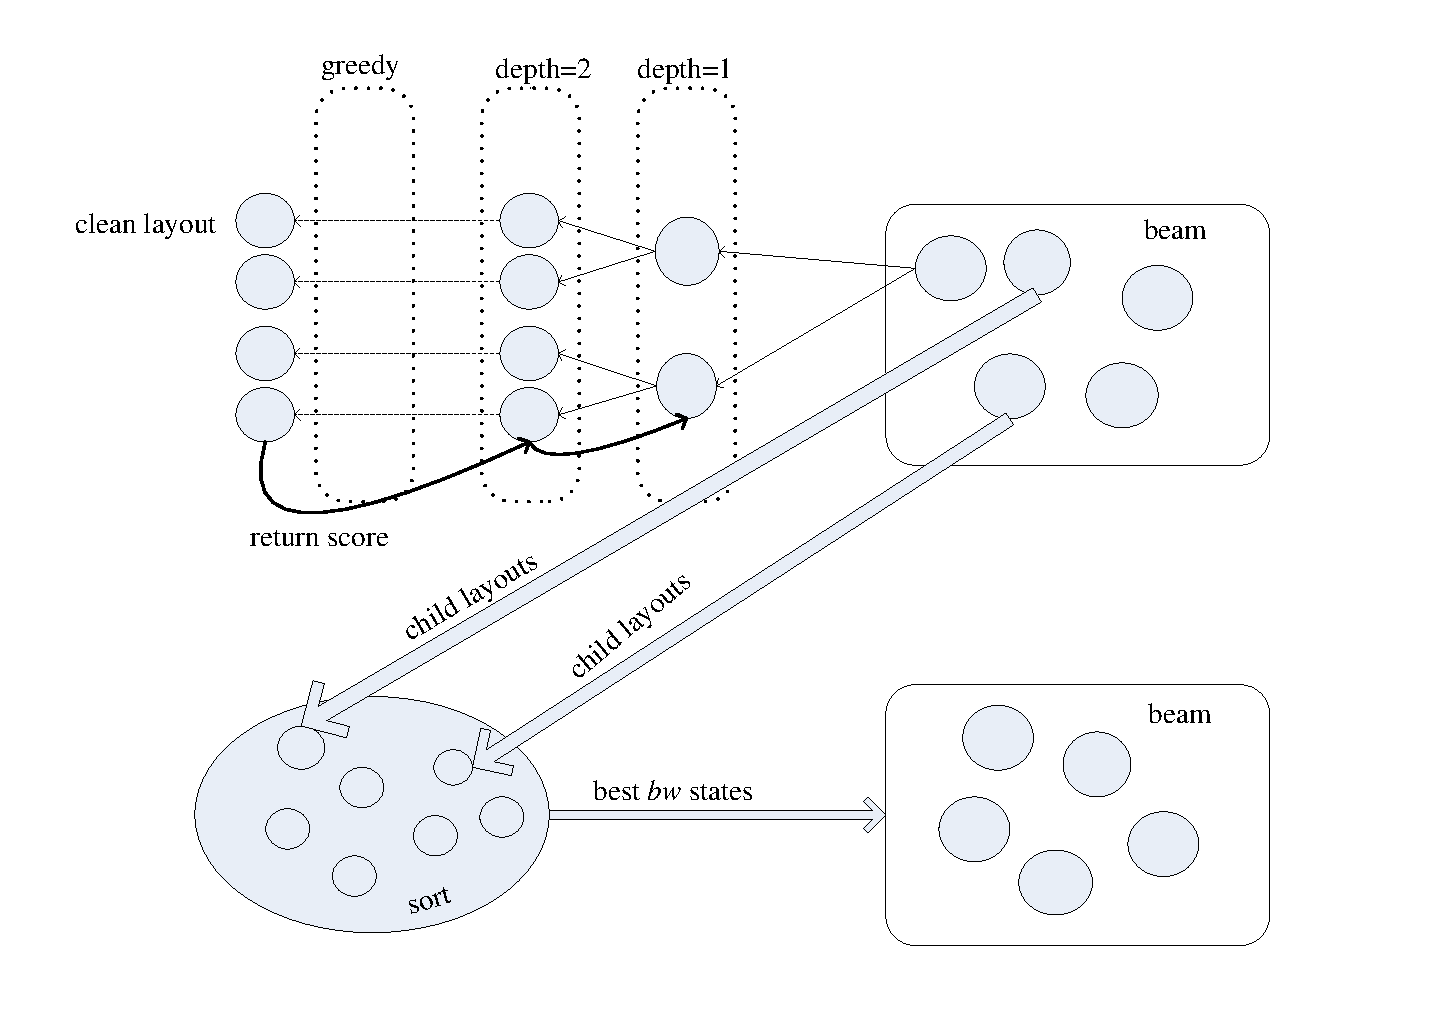
\includegraphics[width=0.4\textwidth]{fig6.pdf}
%\caption{Beam search with giant moves}
%\label{fig6}
%\end{figure*}

\begin{algorithm}[htbp]
	\caption{Beam search with giant moves for the CPMP/CPMPDS}
	\label{alg:bsg}
	\begin{codebox}
	\Procname{\proc{BS-G (\id{inilay})}}
    \li $\id{beam} = \{\id{inilay}\}$
    \li \While ($\id{beam} \neq \emptyset$)
    \li \Do
        $\id{canlaylist}=\emptyset$
    \li \For each \id{lay} in \id{beam}
    \li     \Do
             generate up to $\id{tw}$ children of \id{lay} and append the children to \id{canlaylist}
             \End
    \li     sort the layouts in \id{canlaylist} in a descending order of scores
    \li     \id{beam} = the first $\id{bw}$ layouts in \id{canlaylist}
        \End
	\end{codebox}	
\end{algorithm}

\subsection{Beam search with baby moves}

Inspired by the idea of BS-G, we modify its successor generation method and obtain another algorithm for the CPMP. In this algorithm, beam search is again deployed to maintain the diversity of layouts. The difference from BS-G is that the successors in the beam are generated by applying only a baby move, hence the name beam search with baby moves (BS-B). BS-B overcomes the shortcoming of BS-G that moving too far away (a giant move) each time. Apart from the successor generation method, other components in BS-B is the same with that of BS-G. Now we proceed to introduce how to generate successors in BS-B.

For each layout $l$ in the beam, apply the probing tree search to $l$ just as described in BS-G, generating $\id{tw}$ children. The score of a child is the minimum score of the clean layouts expanded from that child. For each child $\id{child}$ of $l$, BS-B records the first interim layout on the path from $l$ to $\id{child}$ and mark the score of this interim layout the same as the score of $\id{child}$. If an interim has multiple scores because multiple children have it as the first interim layout, then select the smallest score as its score. The successors of $l$ in BS-B are such interim layouts, instead of the children of $l$.

\subsection{Discussion on the CPMPDS}
In this paper, we propose three interrelated algorithms: TGH, BS-G and BS-B. All these algorithms can be applied to solve the CPMP and the CPMPDS instances. Existing algorithms for the CPMP can not be applied directly to solve the CPMPDS instances because they cannot guarantee that the dummy stack is empty when the bay is clean. If we ignore the dummy stack and solve a CPMPDS instance by existing CPMP algorithms, there may not exist a feasible solution.
\section{Experiments and analysis}
\label{sec:ce}
To evaluate the effectiveness of our algorithms, we test our algorithms against the benchmark test data sets provided by \cite{BF2012}.
We first conduct a series of experiments to evaluate the performance of the algorithm components -- the evaluation scheme and search parameters.
It is followed by the performance on the bench mark data.
At the last of this section, a data set for the new CPMPDS is generated and the result is presented for further reference. All of our experiments were conducted on a PC with Intel Core i7 CPU clocked at 3.40 GHz. The operating system is Windows 7.

\subsection {Lower bound comparison}
We use the data of {\em BF2012} to compare the performance of $LB_{DFS}$, $LB_{MKM}$ with that of \cite{BF2012}. In Table \ref{tab:lowerbound}, BF$n$ denotes the $n$th group data. $DFS$, $MKM$ and $BF$ are the average lower bound numbers of the 20 instances in a group calculated by $LB_{DFS}$, $LB_{MKM}$ and \cite{BF2012}, receptively. As such, $T_D$, $T_M$ and $T_B$ are the average computation time of three lower bounds on instances of a group. It can be seen that $DFS$ and $MKM$ dominate $BF$ and the computation time does not increase.
\begin{table}[htbp]
\centering
\caption{\label{tab:lowerbound} Lower Bound Comparison}
\begin{tabular}{c|c|c|c|c|c|c|c|c|c|c|c|c|c}
\hline
      &   BF1  &  BF2   &  BF3  &  BF4  &  BF5  &  BF6  &  BF7  &  BF8 &  BF9 &BF10&BF11&BF12\\
\hline
MKM   & 93.89  & 93.89  &	 0.0& sBR1  & **&&&&&&&\\
%T_M   & 94.48  & 94.57  &	 0.0& sBR4  &\\
%BF& 92.55  & 92.93  &	 0.3& sBR7\ &(2) \\
%T_B   &        &        &       &
%DFS
%T_D
\hline
\end{tabular}
\end{table}

\subsection {Parameter configuration}
\label{sub:config}

In this section, we describe the experiment that reveals the effectiveness of the evaluation scheme as well as the experiments which show how the parameters affect the algorithm performance. These experiments were preliminary testing we performed in order to determine the final configuration of our BS-G and BS-B. We select the data set {\em BF} as our test objective. The data set {\em BF} is generated by \cite{BF2012} and includes 32 groups of instances, denoted by BF1, \dots, BF32; each group of {\em BF} data contains 20 instances for a total of 640 {\em BF} instances. In their instances, the number of stacks is either 16 or 20, and the stack height is either 5 or 8. And they do not have dummy stacks. To avoid over-fitting our algorithms to the benchmark data, we only tested on the first 5 instances of each data group.

We first investigate the effectiveness of different evaluation schemes. As there are other parameters such as the probing tree width and depth, as well as the beam width, we select several combinations of such parameters to make the experiment more robust.

Three kinds of evaluation schemes were tested in our experiment. The first alternative is to evaluate candidate pair by $f(c,s)$ function plus randomness, denoted as \texttt{smallF-ran}. When the pairs have the same $f$ function, randomly select one pair. The second alternative (named \texttt{smallF-lowT}) prefers small $(f(c,s),h(s)-\id{uf}(s))$ which is the one just used in TGH, BS-G and BS-B. The last alternative \texttt{smallF-largeS}, as implied by its name, prefers small $f(c,s)$ and then large $\id{sum}$. Here $\id{sum}$ is the sum of group labels of containers above the target container if the target container and stack are within the same stack; or $\id{sum}$ is the sum of group labels of containers above the target container, in conjunction with those unfixed containers in the target stack.

We tested the three evaluation schemes only against BS-G and set the probing tree width equal to the beam width. The result is shown in Figure \ref{fig7}. The column $w=5$ \& $d=2$ means the probing tree and beam widths are set 5 while the probing tree depth is set 2. The meanings of other columns are similar. Each bar in the chart is the average movements of the test instances. From the experiment, we can see that \texttt{smallF-lowT} has the best performance, \texttt{smallF-ran} ranks the second, then \texttt{smallF-largeS}. The intention of \texttt{smallF-lowT} is to fix target containers lower. And the intention of \texttt{smallF-largeS} is to relocate containers with large group labels earlier. As the results with all the parameter combinations show \texttt{smallF-lowT} outperforms \texttt{smallF-largeS}, the former is indeed better. This can be explained as fixing containers in lower tiers makes the fixed heights among stacks even, namely, containers are fixed, to some extent, tier by tier. This can avoid containers with small group labels occupying short stacks, forcing the slots above them to store only dirty containers. On the contrary, relocating containers with large group labels when there exist larger groups unfixed is not that necessary, or even redundant as the performance is even worse than \texttt{smallF-ran}. The finding indirectly reflects that our ``fix large group first" strategy is reasonable and effective.
\begin{figure*}[htbp]
\centering
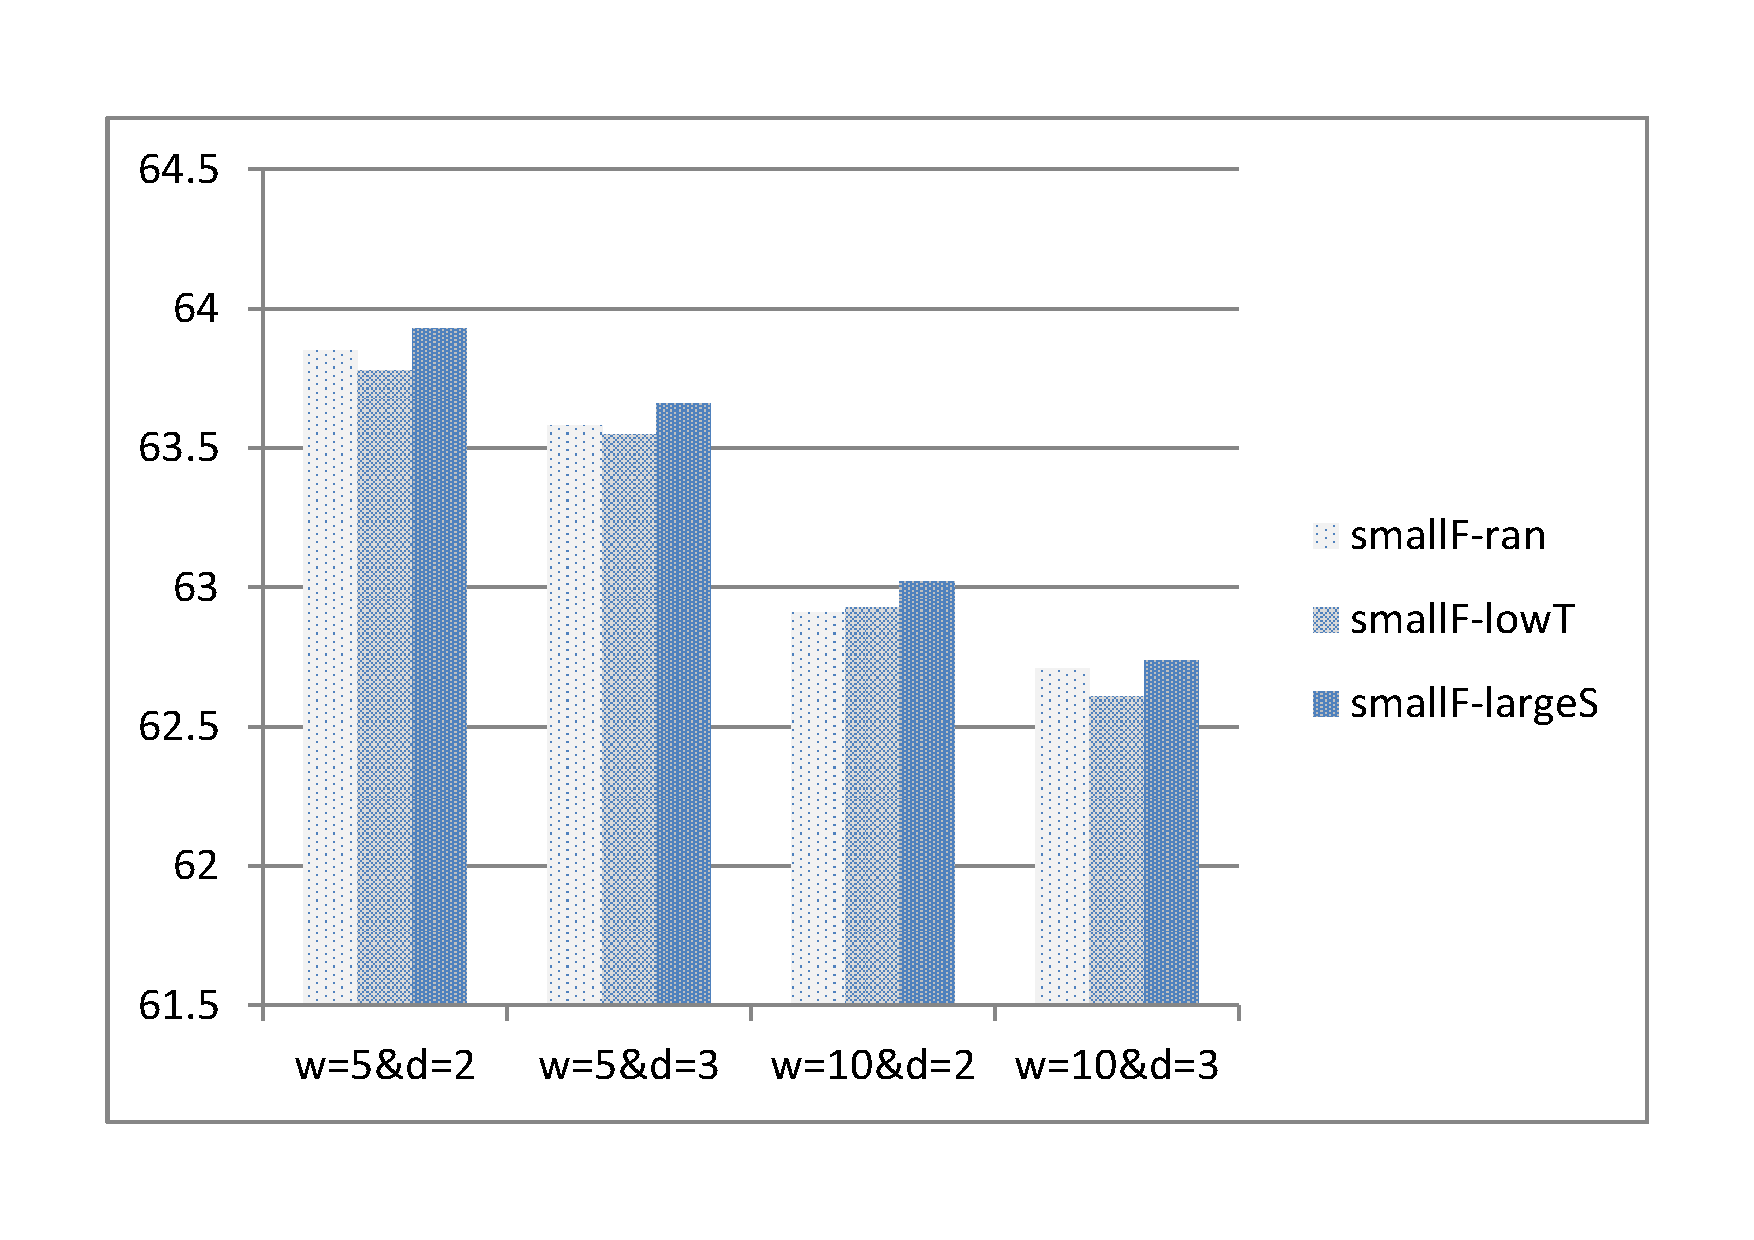
\includegraphics[width=0.4\textwidth]{fig7.pdf}
\caption{Effectiveness of evaluation schemes}
\label{fig7}
\end{figure*}
%\begin{table}[htbp]
%\centering
%\caption{\label{tab:eva_fun} Effect of evaluation function}
%\begin{tabular}{c|c|c|c|c}
%\hline
%Eva Fun      &  $w=5\&d=2$ &  $w=5\&d=3$ & $w=10\&d=2$  & $w=10\&d=3$\\
%\hline
%smallf-ran   &     63.85   &    63.58    &	  62.91     & 62.71\\
%smallf-lowt  &     63.78   &    63.55    &	  62.93     & 62.61\\
%smallf-larges&     63.93   &    63.66    &	  63.02     & 62.74 \\
%\hline
%\end{tabular}
%\end{table}



We next consider the impact of the probing width and depth and the beam width on the algorithm performance. In this experiment, the evaluation scheme is set to be \texttt{smallF-lowT}. To reduce the number of parameter combinations, we once again set the probing tree width equal to the beam width, varying from 2 to 20. We neglect $w=1$ because algorithms deteriorate to TGH when the width equals 1. In addition, the computational time increases exponentially when the probing depth tree increases, thus we only set the depth to be 1, 2, 3, and 4. The data set {\em BF} is classified into four categories based on characteristics: the number of stacks and stack heights (refer to Table \ref{tab:bf}). The first category is the first eight data groups BF1$\sim$BF8 which have 16 stacks and 5 tiers in each instance. Then the second category is BF9$\sim$BF16 with 16 stacks and 8 tiers in each instance. In the following, the third category BF17$\sim$BF24 has 20 stacks and 5 tiers in each instance. At last, the fourth category BF25$\sim$BF32 has 20 stacks and 8 tiers in each instance.
%Again, only the first five instances of each group are tested.

The performance of BS-G on the four categories is separately shown in Figure \ref{fig8:1}$\sim$\ref{fig8:4}. In each figure, it shows the average movements of the corresponding data category obtained by BS-G for different widths and depths. The results of four categories in general have the same trend. When the widths and depths increase, the performance increases, but the improvement becomes smaller and smaller, until in the end diminishes. Furthermore, the performance of $d=2$, $d=3$ and $d=4$ are similar, even the same, indicating that our successor generation method is considerably precise. Compare Figure \ref{fig8:1}$\sim$\ref{fig8:2} with \ref{fig8:3}$\sim$\ref{fig8:4}, it reveals that the performance difference by different parameter combinations for BF1$\sim$BF8 and BF17$\sim$BF24 is tiny while the performance difference by different parameter combinations for BF9$\sim$BF16 and BF25$\sim$BF32 is large. In essence, BF1$\sim$BF8 and BF17$\sim$BF24 are almost solved to the optimality even with a small depth and width. Remind that BF1$\sim$BF8 and BF17$\sim$BF24 are with $H=5$ while BF9$\sim$BF16 and BF25$\sim$BF32 are with $H=8$; all the categories have the same usage ratio. It suggests that the height limit affects the instance difficulty more than the number of stacks. This observation is understandable as containers piled vertically are much harder to be retrieved than those piled horizontally. %When the usage ratio equals, the instance with larger stack height is undoubtedly harder than the instance with larger stack numbers.

\begin{figure}[htbp]
\centering
\subfigure[BF1$\sim$8 average]{
    \label{fig8:1}
    \resizebox{0.4 \textwidth}{!}{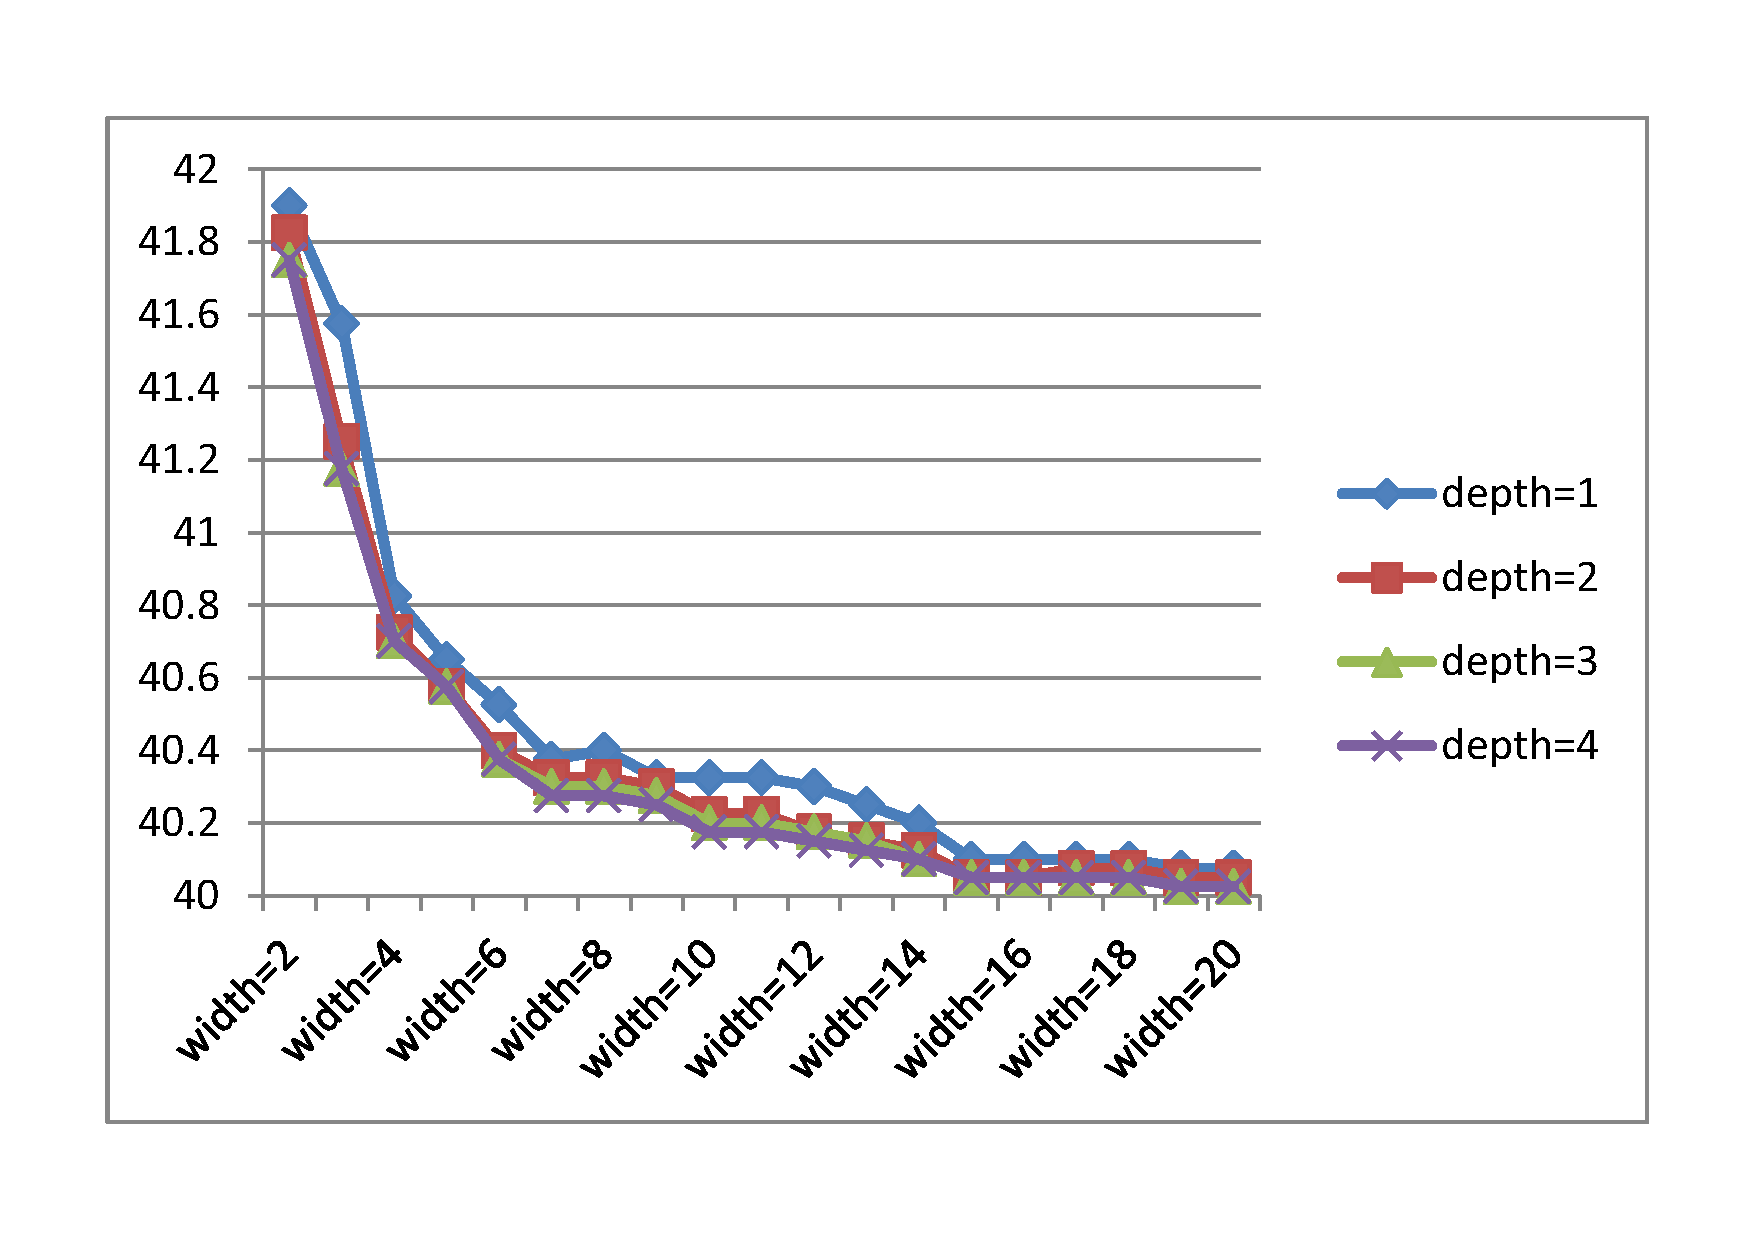
\includegraphics{fig8_1.pdf}}}
\subfigure[BF17$\sim$24 average]{
    \label{fig8:2}
    \resizebox{0.4 \textwidth}{!}{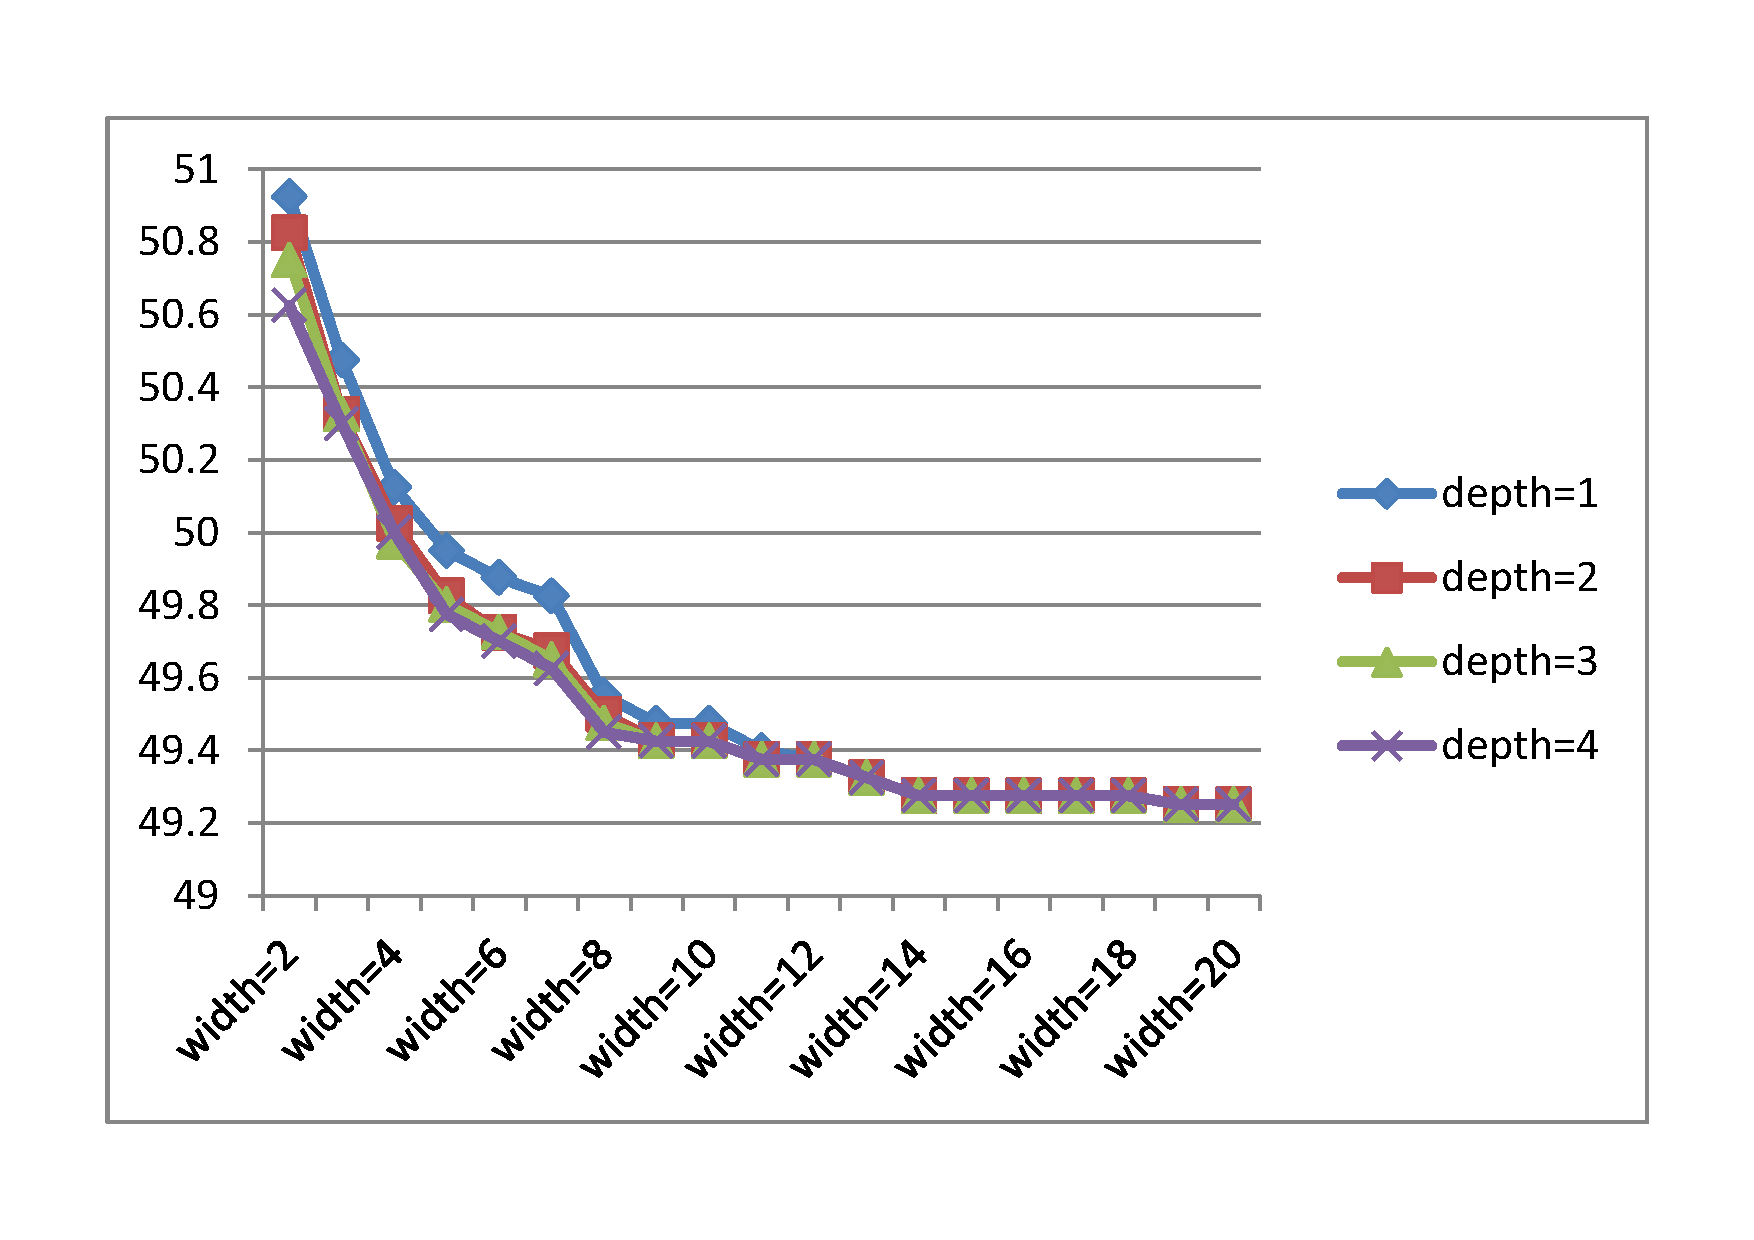
\includegraphics{fig8_2.pdf}}}
\subfigure[BF9$\sim$16 average]{
    \label{fig8:3}
    \resizebox{0.4 \textwidth}{!}{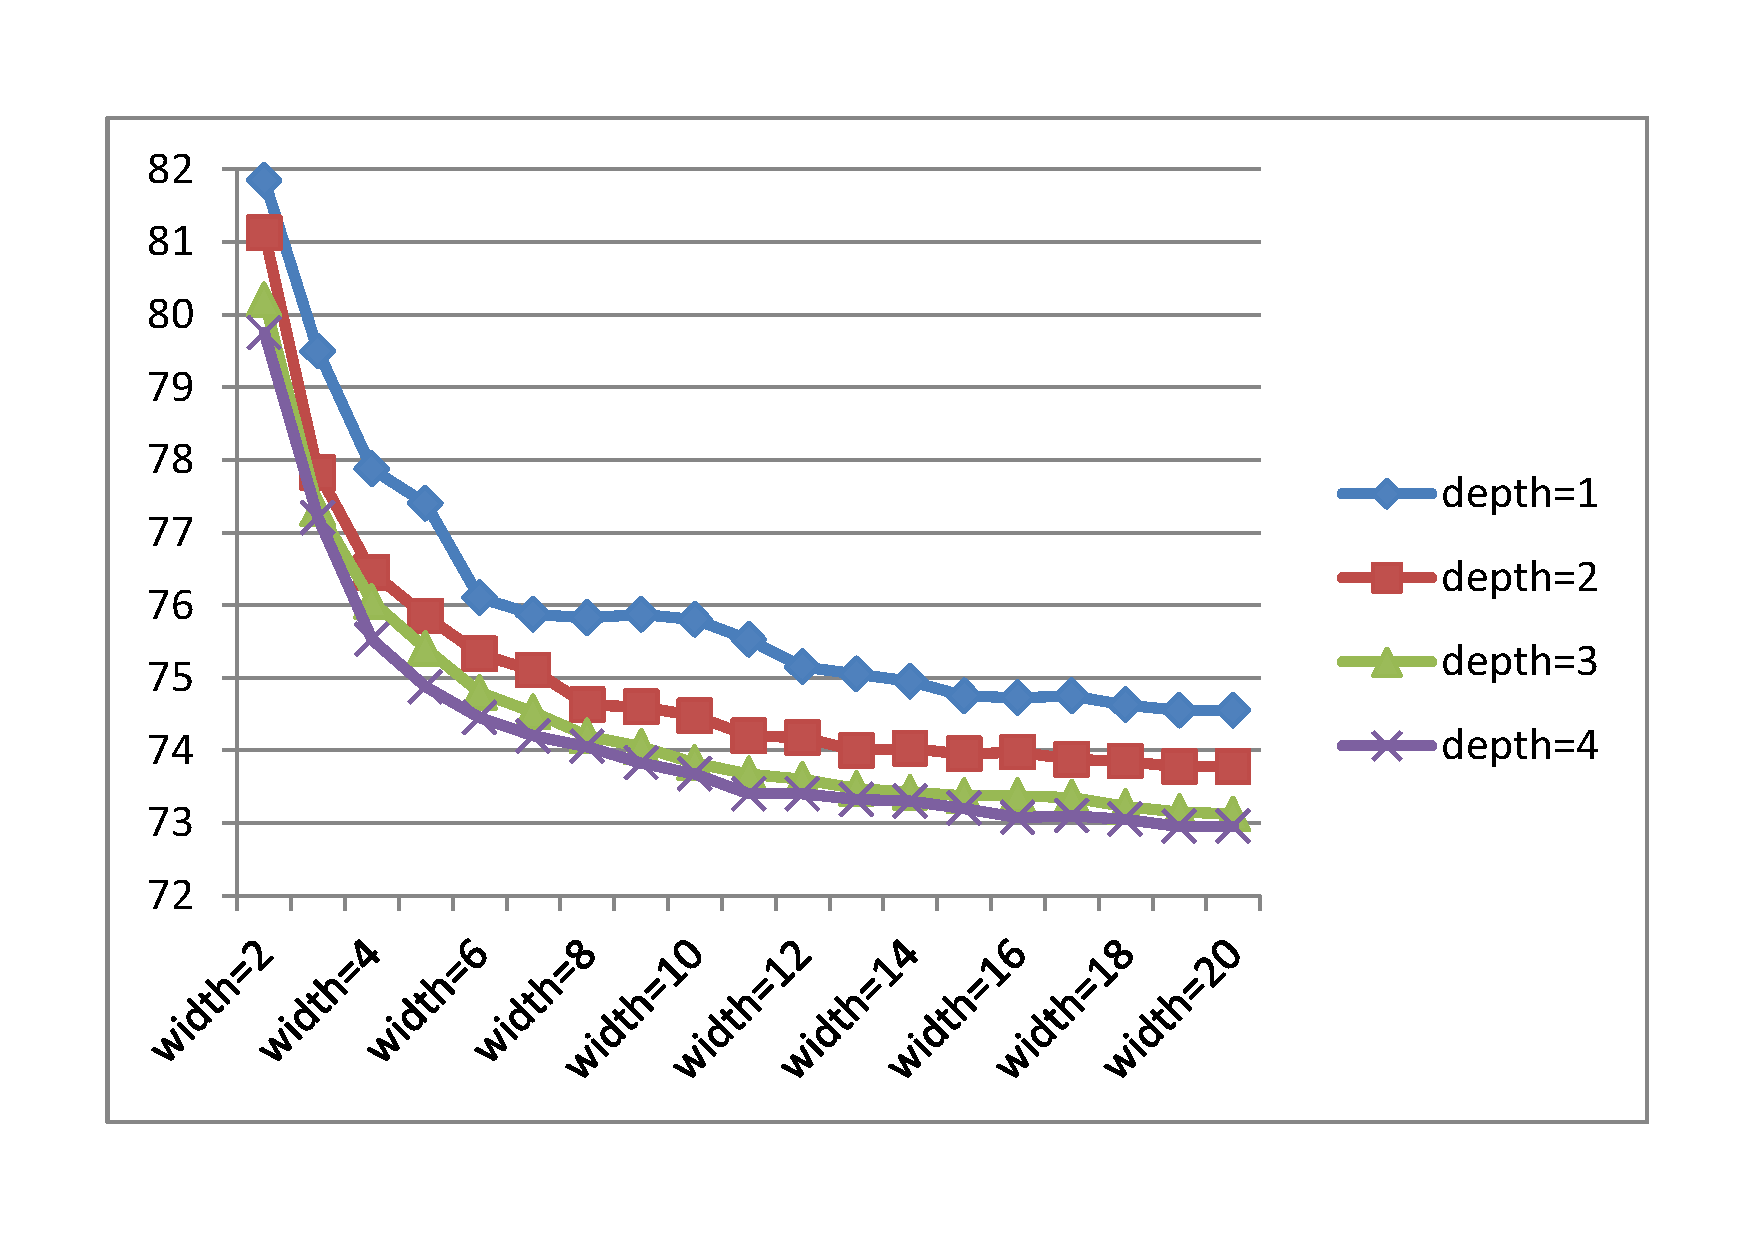
\includegraphics{fig8_3.pdf}}}
\subfigure[BF25$\sim$32 average]{
    \label{fig8:4}
    \resizebox{0.4 \textwidth}{!}{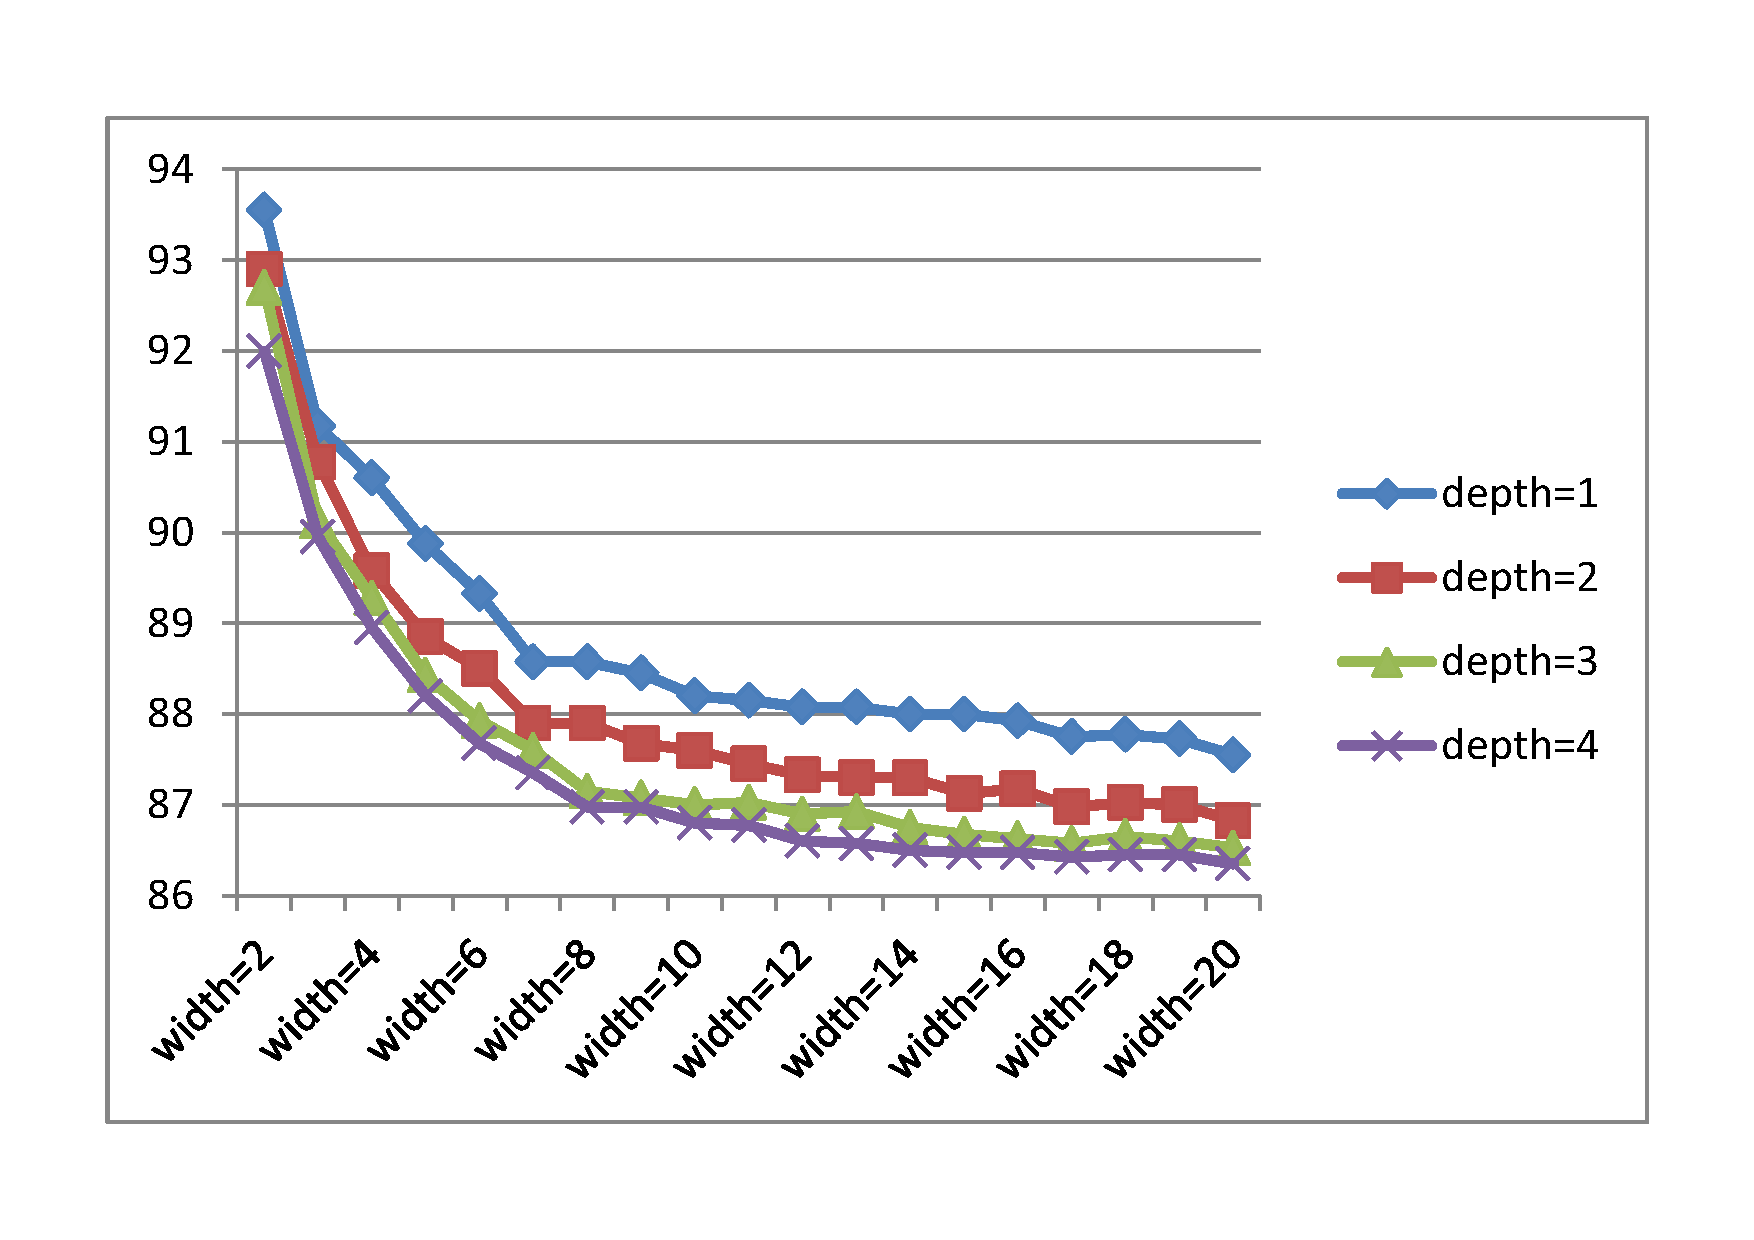
\includegraphics{fig8_4.pdf}}}
\caption{The effect of search depth and width on BS-G}
\label{fig8}
\end{figure}

The performance of BS-B on the four categories are displayed in Figure \ref{fig9}; its trend is similar with that of BS-G in Figure \ref{fig8}, namely the algorithm becomes stable and the improvement is little as parameters enlarge. However, from Figure \ref{fig9}, it can be seen that sometimes the performance goes back when parameters enlarge, especially when the depth is small. For example, in Figure \ref{fig9:4}, the performance when $w=8$ \& $d=1$ is better than the performance when $w=10$ \& $d=1$. The explanation is when $d=1$, the algorithm degenerates to evaluate successors by TGH. The smaller the depth, the weaker ability we have to evaluate successors, therefore more performance deterioration. When the depth increases, performance deterioration disappears. The conclusion is that the heuristic TGH alone is not enough to precisely evaluate successors, and incorporating probing tree search is effective.
\begin{figure}[htbp]
\centering
\subfigure[BF1$\sim$8 average]{
    \label{fig9:1}
    \resizebox{0.4 \textwidth}{!}{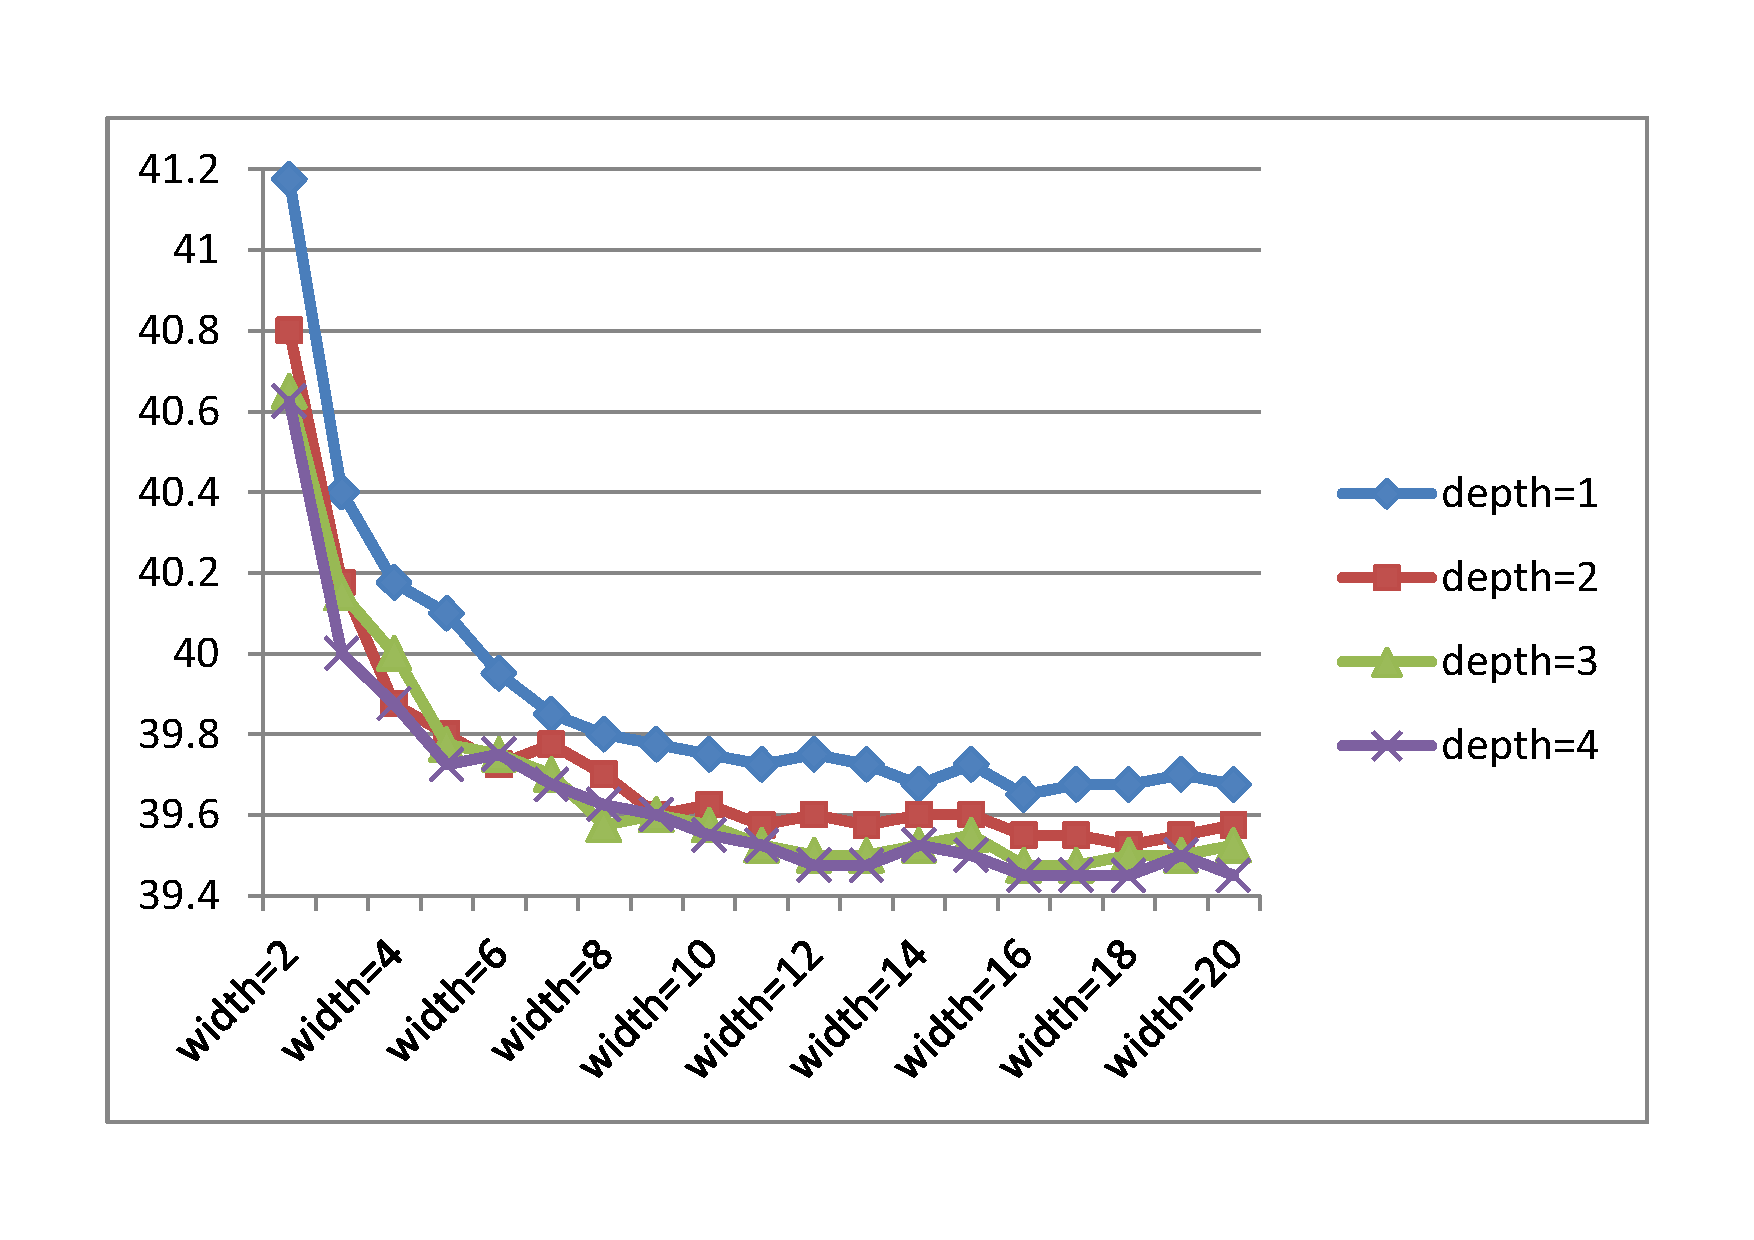
\includegraphics{fig9_1.pdf}}}
\subfigure[BF17$\sim$24 average]{
    \label{fig9:2}
    \resizebox{0.4 \textwidth}{!}{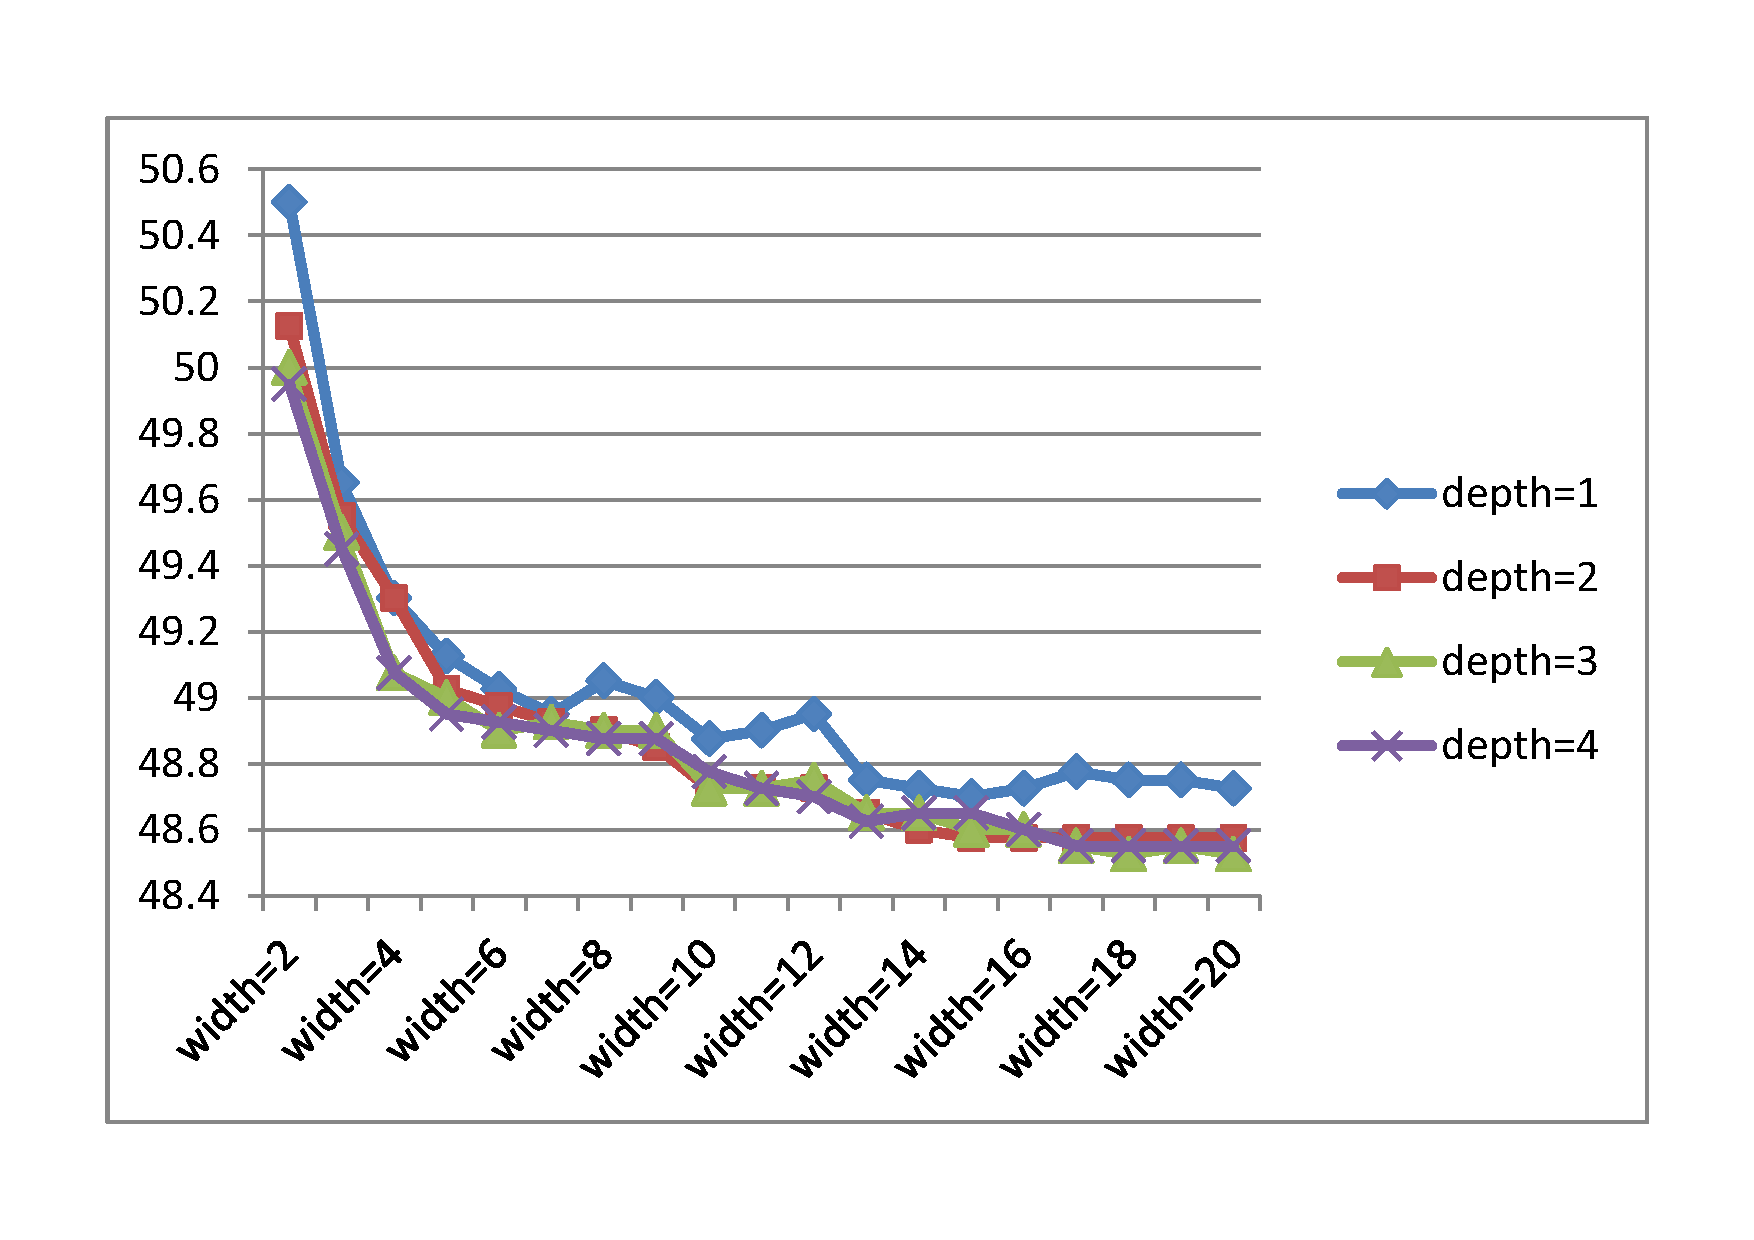
\includegraphics{fig9_2.pdf}}}
\subfigure[BF9$\sim$16 average]{
    \label{fig9:3}
    \resizebox{0.4 \textwidth}{!}{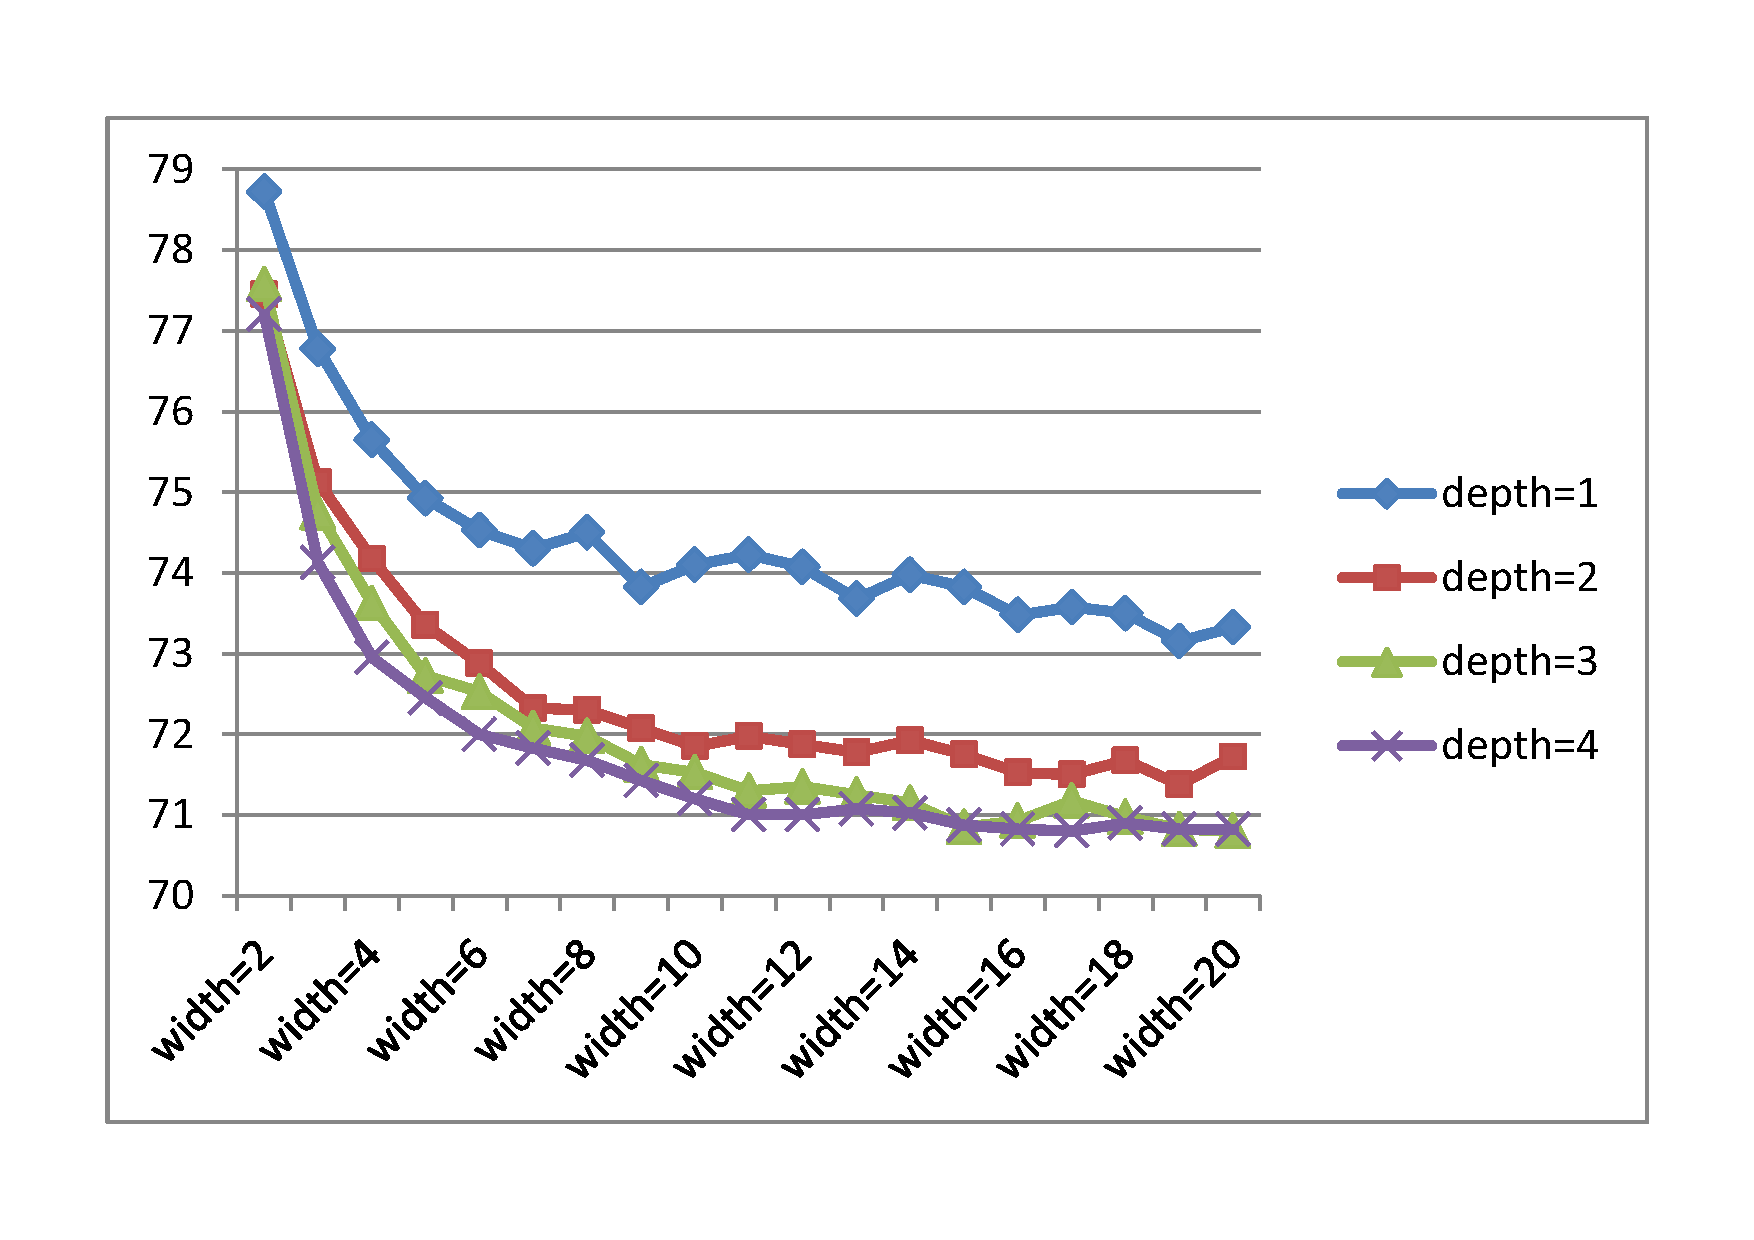
\includegraphics{fig9_3.pdf}}}
\subfigure[BF25$\sim$32 average]{
    \label{fig9:4}
    \resizebox{0.4 \textwidth}{!}{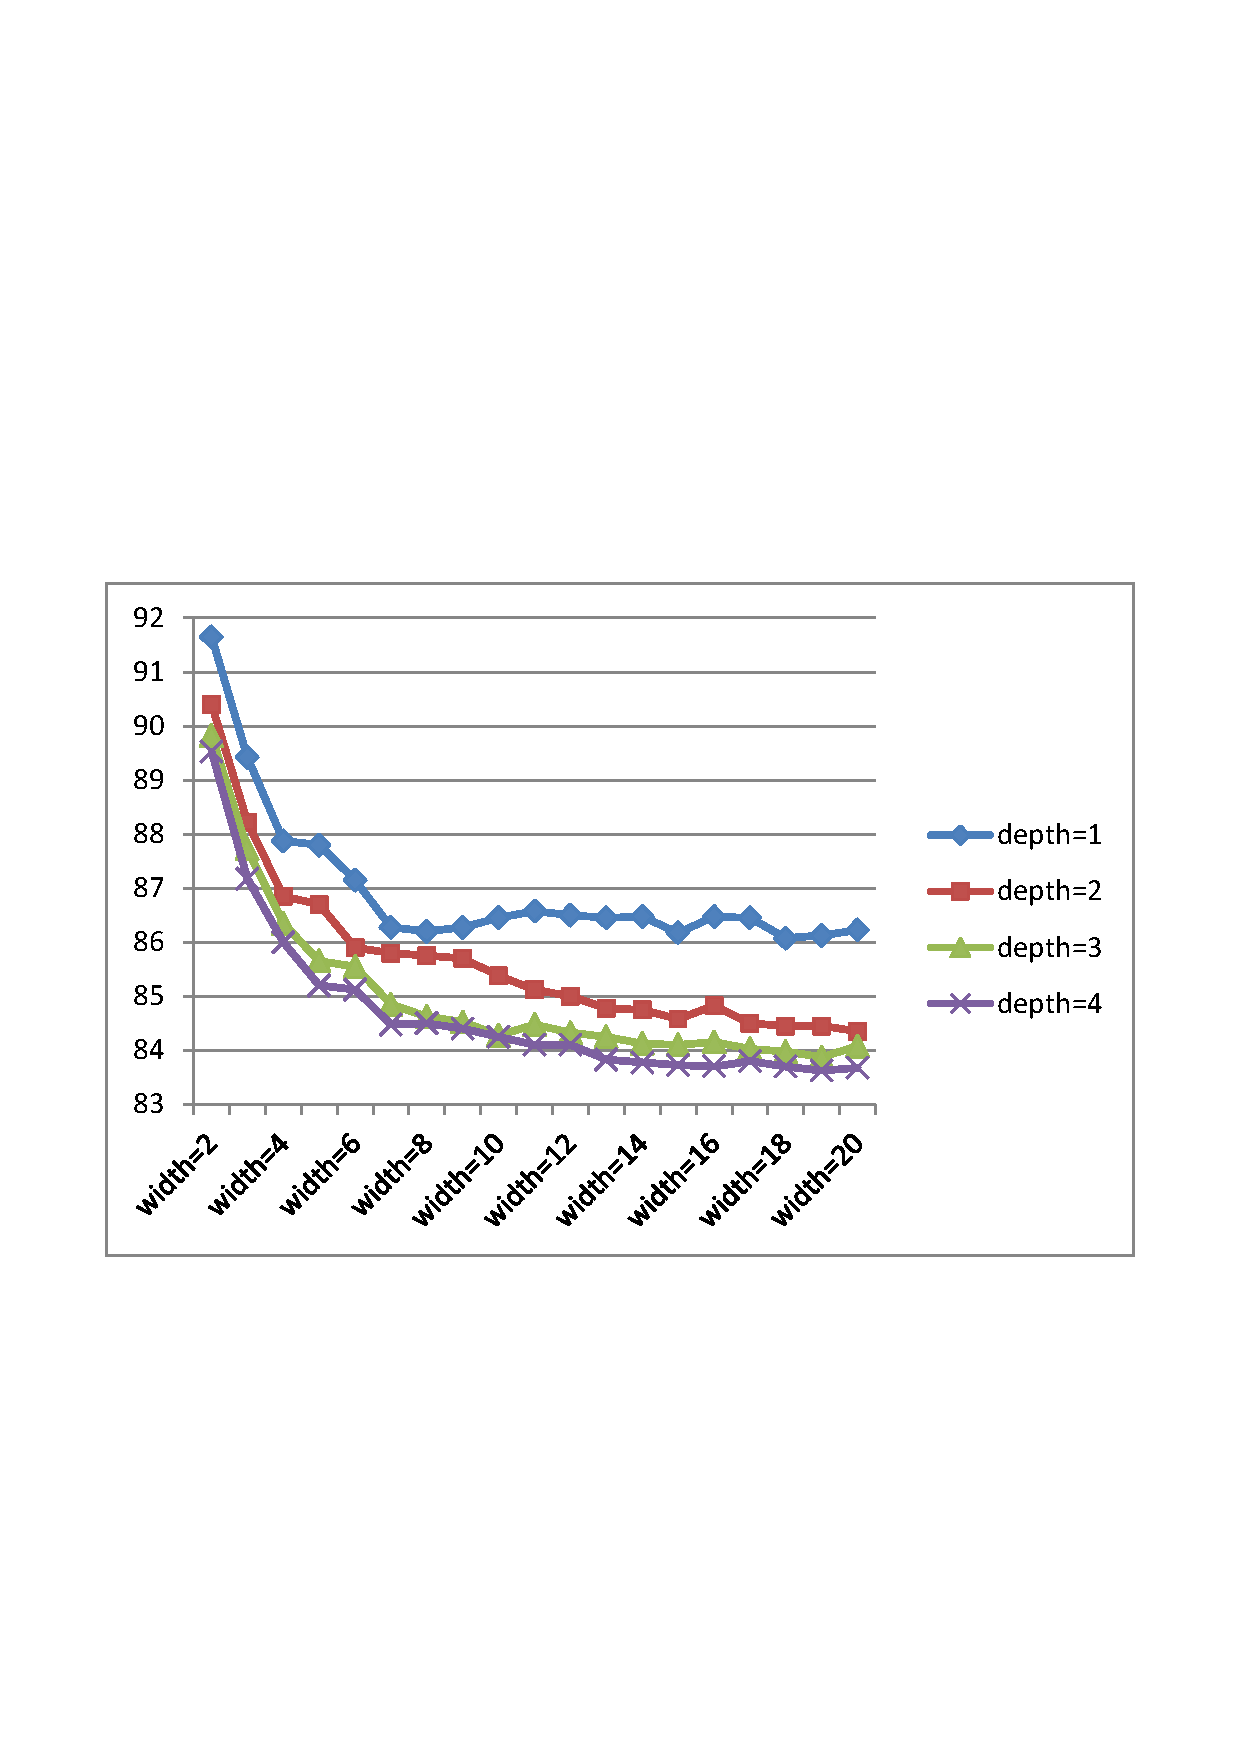
\includegraphics{fig9_4.pdf}}}
\caption{The effect of search depth and width on BS-B}
\label{fig9}
\end{figure}

\subsection {Comparative analysis with CPMP benchmark data}

We compare our algorithms with the tree search algorithm of \cite{BF2012} (BF2012 for short) on the CPMP benchmark data. As far as we know, BF2012 has the best performance on the CPMP. The environment of BF2012 is Intel Core 2 Duo processor (P7350, 16 GFLOPS) with 2 GHz and 2 GB RAM under Mac OS X and their code is written in C and compiled with XCode under Mac OS X. Both the parameters of BS-G and BS-B are set $\id{bw}=\id{tw}=20$ and $\id{td}=3$, since as shown in Figure \ref{fig8} and Figure \ref{fig9}, BS-G and BS-B become stable and the improvement is little if further enlarging the parameters. All the results show two decimal places.

To begin with, we show the result on the data set {\em LC} which is mentioned in Section 7.2 of \cite{BF2012}. The data set {\em LC} is first generated by \cite{Lee2009}, but their concrete data set is not available. For this reason, \cite{BF2012} generate a new set of instances according to the description of \cite{Lee2009}. The result on data set {\em LC} is displayed in Table \ref{tab:lc}. The first five columns of Table \ref{tab:lc} summarise the data information copied from \cite{BF2012}, out of which the dirty ratio is the number of dirty containers in the initial layout divided by the number of containers.
The column BF2012, TGH, BS-G and BS-B are the average movements on each data group by algorithms BF2012, our TGH, our BS-G and BS-B receptively. The average run time by BF2012, BS-G and BS-B are reported in column tBF2012, tBS-G and tBS-B, in unit of second. As the run time of TGH is less than 0.2s, we do not report its run time in the table. In the last row of the table, we also give the mean movements on the whole {\em LC} data. The average time takes cells with ``$<1$''  as 1s and cells with ``$<0.1$" as 0.1s. We highlight results on which our algorithms outperform BF2012 in bold. Our algorithm TGH and BS-G are worse than BF2012, while BS-B is better than BF2012, but the improvement is little. We explain this phenomenon as the size of the test instances is small and BF2012 has almost solved the instances to the optimality.
\begin{table}[htbp]
\begin{footnotesize}

  \caption{\label{tab:lc} Algorithms comparison on data set {\em LC}}
    \begin{tabular}{c|c|c|c|c|c|c|c|c|c|c|c}

    \hline
    group & stack & height & usage rate & dirty ratio & BF2012 & tBF2012 & TGH   & BS-G  & tBS-G & BS-B  & tBS-B \\
    \hline
    LC1   & 10  & 5  & 0.70  & 0.37  & 17.00  & $<1$  & 22.00  & 17.00  & $<0.1$  & 17.00  & $<1$ \\
    LC2a  & 12  & 6  & 0.69  & 0.38  & 22.60  & 1.00  & 26.90  & 23.20  & $<0.1$  & \textbf{22.30}  & $<1$ \\
    LC2b  & 12  & 6  & 0.69  & 0.70  & 38.40  & 2.10  & 46.70  & \textbf{38.00}  & $<0.1$  & \textbf{37.90}  & 1.37  \\
    LC3a  & 12  & 6  & 0.75  & 0.39  & 23.70  & 1.40  & 29.10  & 23.90  & $<0.1$  & 23.70  & $<1$ \\
    LC3b  & 12  & 6  & 0.75  & 0.67  & 42.70  & 4.20  & 54.80  & 43.60  & $<1$    & \textbf{42.30}  & 10.33  \\
    \hline
    Ave   & 11.60  & 5.80  & 0.72  & 0.50  & 28.88  & 1.94  & 35.90  & 29.14  & $<1$    & \textbf{28.64}  & 2.69  \\
    \hline
    \end{tabular}%
\end{footnotesize}
\end{table}%

Then we compare our algorithms with BF2012 on data set {\em CV}. The data set {\em CV} is provided by \cite{Caserta2009} and by far \cite{BF2012} has the best performance on this data set. Table \ref{tab:cv} reports the comparative result on the data set {\em CV}. It can be seen that both BS-G and BS-B surpass the BF2012.
\begin{table}[htbp]
\begin{footnotesize}
  \centering
  \caption{\label{tab:cv} Algorithms comparison on data set {\em CV}}
    \begin{tabular}{c|c|c|c|c|c|c|c|c|c|c|c}
    \hline
    group & stack & height & usage rate & dirty ratio & BF2012 & tBF2012 & TGH   & BS-G  & tBS-G & BS-B  & tBS-B \\
    \hline
    CV1   & 3  & 9  & 0.33  & 0.60  & 10.50  & $<1$    & 12.10  & 10.60  & $<0.01$ & \textbf{10.00}  & $<0.01$ \\
    CV2   & 4  & 16 & 0.25  & 0.66  & 19.10  & $<1$    & 20.30  & \textbf{17.80}  & $<0.01$ & \textbf{17.20}  & $<0.1$ \\
    CV3   & 5  & 25 & 0.20  & 0.70  & 30.40  & 9.10    & 34.00  & \textbf{27.30}  & $<0.1$  & \textbf{26.40} & $<1$ \\
    CV4   & 6  & 36 & 0.17  & 0.74  & 44.40  & 20.00   & 50.00  & \textbf{37.10}  & $<0.1$  & \textbf{35.90}  & $<1$ \\
    \hline
    Ave   & 4.50  & 21.50 & 0.24  & 0.67  & 26.10  & 7.78    & 29.10  & \textbf{23.20}  & $<0.1$  & \textbf{22.38}  & $<1$ \\
    \hline
    \end{tabular}%
\end{footnotesize}
\end{table}%

 At last we display the results on the data set {\em BF} by different algorithms in Table \ref{tab:bf}. The data set {\em BF} is generated by \cite{BF2012} and they claim that the instances are difficult enough to justify the performance of algorithms. For TGH, its performance is worse than that of BF2012. This is understandable because BF2012 deploys a tree search algorithm whereas TGH is only a greedy heuristic. BS-G outperforms BF2012 by almost 5\%, and BS-B outperforms BF2012 by almost 7\%.  What's more, the computational time of BS-G is less than that of BF2012. Although the computational time of BS-B is much more than that of BF2012 in Table \ref{tab:bf}, the results are still better than that of BF2012 if we decrease parameters to make run the time of BS-B close to the run time of BF2012.

\begin{table}[htbp]
\caption{\label{tab:bf} Algorithms comparison on data set {\em BF}}
\footnotesize
\begin{tabular}{c|c|c|c|c|c|c|c|c|c|c|c}
  \hline
  group & stack & height & usage rate & dirty ratio & BF2012 & tBF2012 & TGH   & BS-G  & tBS-G & BS-B  & tBS-B \\
    \hline
    BF1   & 16    & 5     & 0.6   & 0.60  & 29.10  & $<1$  & 29.10  & 29.10  & $<0.01$ & 29.10  & $<0.01$ \\
    BF2   & 16    & 5     & 0.6   & 0.75  & 36.00  & $<1$  & 36.00  & 36.00  & $<0.01$ & 36.00  & $<0.01$ \\
    BF3   & 16    & 5     & 0.6   & 0.60  & 29.10  & $<1$  & 29.45  & 29.15  & $<0.01$ & 29.10  & $<0.1$ \\
    BF4   & 16    & 5     & 0.6   & 0.75  & 36.00  & $<1$  & 36.00  & 36.00  & $<0.01$ & 36.00  & $<0.01$ \\
    BF5   & 16    & 5     & 0.8   & 0.61  & 41.60  & 8.00  & 48.25  & 42.05  & $<0.1$  & \textbf{41.35}  & 3.73  \\
    BF6   & 16    & 5     & 0.8   & 0.75  & 49.40  & 4.90  & 57.65  & 51.10  & $<0.1$  & 50.15  & 10.87  \\
    BF7   & 16    & 5     & 0.8   & 0.61  & 42.90  & 26.30 & 53.50  & 44.75  & $<0.1$  & 43.05  & 8.95  \\
    BF8   & 16    & 5     & 0.8   & 0.75  & 50.60  & 24.70 & 60.05  & 51.95  & $<0.1$  & 51.15  & 15.75  \\
    BF9   & 16    & 8     & 0.6   & 0.61  & 51.80  & 30.80 & 60.35  & \textbf{51.50}  & $<0.1$  & \textbf{50.40}  & 6.87  \\
    BF10  & 16    & 8     & 0.6   & 0.75  & 59.80  & 21.90 & 62.05  & \textbf{58.90}  & $<0.01$ & \textbf{58.75}  & 2.99  \\
    BF11  & 16    & 8     & 0.6   & 0.61  & 52.20  & 44.60 & 61.15  & 52.30  & $<0.1$  & \textbf{51.15}  & 7.75  \\
    BF12  & 16    & 8     & 0.6   & 0.75  & 60.20  & 28.20 & 63.45  & \textbf{59.20}  & $<0.1$  & \textbf{58.65}  & 3.47  \\
    BF13  & 16    & 8     & 0.8   & 0.60  & 84.60  & 60.00 & 107.45 & \textbf{79.75 } & 2.67    & \textbf{75.40}  & 167.50  \\
    BF14  & 16    & 8     & 0.8   & 0.76  & 105.60 & 60.00 & 125.25 & \textbf{96.30}  & 4.62    & \textbf{93.10}  & 293.56  \\
    BF15  & 16    & 8     & 0.8   & 0.60  & 95.50  & 60.00 & 110.90 & \textbf{82.80 } & 2.66    & \textbf{78.70}  & 176.51  \\
    BF16  & 16    & 8     & 0.8   & 0.76  & 109.80 & 60.00 & 133.30 & \textbf{98.00 } & 4.28    & \textbf{93.55}  & 275.25  \\
    BF17  & 20    & 5     & 0.6   & 0.60  & 36.30  & 3.50  & 36.45  & \textbf{36.25 } & $<0.01$ & \textbf{36.25}  & $<0.01$ \\
    BF18  & 20    & 5     & 0.6   & 0.75  & 45.00  & $<1$  & 45.00  & 45.00  & $<0.01$ & 45.00  & $<0.01$ \\
    BF19  & 20    & 5     & 0.6   & 0.60  & 36.50  & $<1$  & 36.80  & 36.50  & $<0.01$ & \textbf{36.45}  & $<0.01$ \\
    BF20  & 20    & 5     & 0.6   & 0.75  & 45.00  & $<1$  & 45.00  & 45.00  & $<0.01$ & 45.00  & $<0.01$ \\
    BF21  & 20    & 5     & 0.8   & 0.60  & 51.70  & 31.50 & 60.80  & 52.45  & $<0.1$  & \textbf{51.55}  & 20.31  \\
    BF22  & 20    & 5     & 0.8   & 0.75  & 60.90  & 7.60  & 68.90  & 62.85  & $<0.1$  & 61.80  & 14.47  \\
    BF23  & 20    & 5     & 0.8   & 0.60  & 51.50  & 25.50 & 60.85  & 52.40  & $<0.1$  & \textbf{50.95}  & 13.90  \\
    BF24  & 20    & 5     & 0.8   & 0.75  & 61.30  & 18.20 & 70.95  & 63.25  & $<0.1$  & 62.05  & 24.45  \\
    BF25  & 20    & 8     & 0.6   & 0.60  & 62.80  & 45.00 & 69.95  & \textbf{62.10 } & $<0.1$  & \textbf{61.50}  & 12.79  \\
    BF26  & 20    & 8     & 0.6   & 0.75  & 74.00  & 30.80 & 74.35  & \textbf{72.60 } & $<0.1$  & \textbf{72.35}  & 2.53  \\
    BF27  & 20    & 8     & 0.6   & 0.60  & 64.00  & 55.90 & 71.80  & \textbf{62.75 } & $<0.1$  & \textbf{61.85}  & 16.12  \\
    BF28  & 20    & 8     & 0.6   & 0.75  & 74.90  & 44.70 & 76.10  & \textbf{73.00 } & $<0.1$  & \textbf{72.65}  & 5.82  \\
    BF29  & 20    & 8     & 0.8   & 0.60  & 106.60 & 60.00 & 120.55 & \textbf{96.05}  & 8.50    & \textbf{92.05}  & 396.10  \\
    BF30  & 20    & 8     & 0.8   & 0.75  & 128.50 & 60.00 & 143.05 &\textbf{ 114.30} & 11.40   & \textbf{110.25} & 581.61  \\
    BF31  & 20    & 8     & 0.8   & 0.60  & 115.20 & 60.00 & 128.15 & \textbf{98.90}  & 9.17    & \textbf{93.95}  & 429.09  \\
    BF32  & 20    & 8     & 0.8   & 0.75  & 132.30 & 60.00 & 147.30 & \textbf{115.55} & 8.32    & \textbf{111.80} & 612.55  \\
    \hline
    Ave   & 18.00 & 6.50  & 0.7   & 0.68  & 65.02  & 29.35 & 72.81  & \textbf{62.12}  & 1.64    & \textbf{60.66}  & 96.97  \\
   \hline
\end{tabular}
\end{table}

\subsection {New data}
We generate a new data set for the CPMPDS. All the data is available at our website\footnote{\url{http://www.computational-logistics.org/orlib/topic/CPMPDS/index.html}}. The new data set is composed of 36 groups of instances, with 30 instances in each group. The number of stacks is 6, 8, or 10 (dummy stack included) as in reality the number of stacks in a bay is in such a range. The maximum height limit is 5 or 8 as it is restricted by the handling equipments in practice. There are two alternatives with respect to the usage rate. One alternative is 60\%$\sim$80\%, and another alternative is 80\% above. Following the spirit of \cite{BF2012}, the number of different group labels in an instance is decided by the group ratio equal to the number of different groups divided by the number of containers. In our data set, the group ratio has three ranges: 100\%, 60\%$\sim$80\%, 30\%$\sim$50\%. Particularly, group ratio 100\% means that the group labels of containers are unique. The results by TGH, BS-G and BS-B are reported in Table \ref{tab:cpmpds}.

\begin{table}[htbp]

\caption{\label{tab:cpmpds} Results for the data set {\em CPMPDS}}
\footnotesize
\centering
\begin{tabular}{c|c|c|c|c|c|c|c|c|c}

    \hline
    group & stack & tier  & usage rate & dirty ratio & TGH   & BS-G  & tBS-G & BS-B  & tBS-B \\
    \hline
    CPMPDS1 & 6      & 5     & 0.70  & 0.57  & 29.33   & 21.13  & $<0.1$  & 19.97  & $<1$ \\
    CPMPDS2 & 6      & 5     & 0.72  & 0.62  & 33.10   & 23.30  & $<0.1$  & 21.97  & $<1$ \\
    CPMPDS3 & 6      & 5     & 0.69  & 0.53  & 23.87   & 17.83  & $<0.1$  & 17.37  & $<1$\\
    CPMPDS4 & 6      & 5     & 0.82  & 0.68  & 62.13   & 37.37  & $<0.1$  & 34.33  & $<1$ \\
    CPMPDS5 & 6      & 5     & 0.82  & 0.63  & 55.03   & 33.23  & $<1$    & 30.43  & 1.16  \\
    CPMPDS6 & 6      & 5     & 0.82  & 0.61  & 53.57   & 30.70  & $<1$    & 28.90  & 1.98  \\
    CPMPDS7 & 6      & 8     & 0.68  & 0.73  & 72.97   & 43.73  & $<1$    & 41.00  & 1.23  \\
    CPMPDS8 & 6      & 8     & 0.69  & 0.74  & 74.47   & 45.40  & $<1$    & 42.27  & 2.28  \\
    CPMPDS9 & 6      & 8     & 0.69  & 0.73  & 60.80   & 41.37  & $<1$    & 39.63  & 2.28  \\
    CPMPDS10 & 6     & 8     & 0.80  & 0.78  & 142.73  & 72.00  & $<1$    & 66.93  & 4.05  \\
    CPMPDS11 & 6     & 8     & 0.81  & 0.78  & 157.57  & 72.83  & $<1$    & 68.63  & 6.09  \\
    CPMPDS12 & 6     & 8     & 0.81  & 0.75  & 138.43  & 66.43  & $<1$    & 62.60  & 11.27  \\
    CPMPDS13 & 8     & 5     & 0.71  & 0.60  & 32.47   & 25.30  & $<0.1$  & 24.33  & $<1$ \\
    CPMPDS14 & 8     & 5     & 0.72  & 0.59  & 33.67   & 25.93  & $<1$    & 25.03  & 1.17  \\
    CPMPDS15 & 8     & 5     & 0.68  & 0.55  & 25.40   & 21.17  & $<0.1$  & 20.43  & $<1$ \\
    CPMPDS16 & 8     & 5     & 0.84  & 0.69  & 73.50   & 44.30  & $<1$    & 41.50  & 3.86  \\
    CPMPDS17 & 8     & 5     & 0.83  & 0.64  & 64.67   & 39.00  & $<1$    & 37.47  & 4.85  \\
    CPMPDS18 & 8     & 5     & 0.83  & 0.61  & 53.83   & 35.30  & $<1$    & 33.77  & 5.23  \\
    CPMPDS19 & 8     & 8     & 0.69  & 0.71  & 73.20   & 48.90  & $<1$    & 46.30  & 3.49  \\
    CPMPDS20 & 8     & 8     & 0.70  & 0.72  & 76.43   & 51.97  & $<1$    & 49.43  & 9.31  \\
    CPMPDS21 & 8     & 8     & 0.69  & 0.72  & 70.23   & 49.10  & $<1$    & 47.20  & 9.88  \\
    CPMPDS22 & 8     & 8     & 0.84  & 0.78  & 173.37  & 87.50  & 1.44    & 81.70  & 18.77  \\
    CPMPDS23 & 8     & 8     & 0.85  & 0.78  & 176.23  & 90.37  & 2.31    & 85.73  & 28.55  \\
    CPMPDS24 & 8     & 8     & 0.84  & 0.78  & 153.87  & 82.07  & 3.32    & 78.67  & 48.31  \\
    CPMPDS25 & 10    & 5     & 0.71  & 0.58  & 35.77   & 28.07  & $<1$    & 27.17  & 1.46  \\
    CPMPDS26 & 10    & 5     & 0.69  & 0.58  & 31.20   & 25.77  & $<1$    & 24.87  & 1.44  \\
    CPMPDS27 & 10    & 5     & 0.69  & 0.56  & 30.43   & 25.23  & $<1$    & 24.47  & 2.19  \\
    CPMPDS28 & 10    & 5     & 0.86  & 0.63  & 83.30   & 50.40  & 1.33    & 48.20  & 12.90  \\
    CPMPDS29 & 10    & 5     & 0.85  & 0.64  & 68.70   & 46.30  & 1.18    & 44.17  & 13.09  \\
    CPMPDS30 & 10    & 5     & 0.86  & 0.63  & 71.67   & 44.90  & 2.64    & 42.93  & 22.31  \\
    CPMPDS31 & 10    & 8     & 0.69  & 0.72  & 82.07   & 59.00  & $<1$    & 55.87  & 11.78  \\
    CPMPDS32 & 10    & 8     & 0.70  & 0.71  & 84.63   & 58.40  & 1.12    & 55.97  & 19.15  \\
    CPMPDS33 & 10    & 8     & 0.70  & 0.73  & 77.73   & 57.50  & 1.50    & 55.13  & 23.76  \\
    CPMPDS34 & 10    & 8     & 0.87  & 0.77  & 221.83  & 114.23 & 5.61    & 110.37 & 79.28  \\
    CPMPDS35 & 10    & 8     & 0.85  & 0.77  & 171.73  & 97.70  & 5.49    & 93.03  & 79.78  \\
    CPMPDS36 & 10    & 8     & 0.85  & 0.77  & 172.83  & 95.90  & 9.44    & 91.90  & 158.40  \\
    \hline
    Ave      & 8.00  & 6.50  & 0.77  & 0.68  & 84.52   & 50.27  & 1.18    & 47.77  & 16.46  \\
    \hline
\end{tabular}
\end{table}%




\section{Conclusions}
\label{sec:con}
The container pre-marshalling problem is an important topic at container terminals, and its efficient solution has a significant impact on efficient use of container yards, as well as competition power of container terminals. In particular, the CPMP with a dummy stack has been overlooked by the research community for a long time; whereas in reality terminals using gantry cranes are a lot.
In this paper, we considered the classic container pre-marshalling problem. At the same time, we proposed a new variant CPMP with a dummy stack (CPMPDS). Three algorithms were devised based on the idea of fixing containers one by one to solve both the classic CPMP and CPMPDS. We also came up with a new improved lower bound to compute the number of movements. Experiments showcase that our algorithms outperform existing methods in terms of the benchmark data of the CPMP, and BS-B can be regarded as the current best algorithm for the CPMP/CPMPDS.
In addition, we constructed a new data set of the CPMPDS for future reference .

Through experimental analysis, we find that the idea of fixing containers from larger group labels is right as it narrows the solution space, and provides guidance for the algorithms. The heuristic rules in TGH are also critical as the efficiency of giant moves affects the efficiency of the whole beam search algorithms. The thought of combining giant moves with beam search is also applicable to other complex problems whose solution space are too large to be fully explored.

In the future, we can address which factors affect the difficulty of the CPMP instances and incorporate the CPMP with its upstream and downstream problems, such as stacking problems, cranes scheduling problems and stowage planning problems.




\bibliographystyle{model5-names}
\bibliography{reference}
\end{document}
